\documentclass[lettersize,journal]{IEEEtran}
\usepackage{amsmath,amsfonts,amssymb}
\usepackage{algorithmic}
\usepackage{algorithm}
\usepackage{array}
\usepackage[caption=false,font=normalsize,labelfont=sf,textfont=sf]{subfig}
\usepackage{textcomp}
\usepackage{stfloats}
\usepackage{url}
\usepackage{verbatim}
\usepackage{graphicx}
\usepackage{cite}
\usepackage{booktabs}
\usepackage{makecell}
\usepackage{longtable}
\usepackage{multirow}
\usepackage{color}
\usepackage{hyperref}

\hyphenation{op-tical net-works semi-conduc-tor IEEE-Xplore}

\begin{document}

\title{GS-LSS: Learned Stochastic Sampling for 3D Gaussian Splatting under Biased Viewpoints}

\author{Ao Zhang,
Qiong Liu,~\IEEEmembership{Senior Member,~IEEE}, 
Wenxuan He, Jiabo Wu,
and You Yang,~\IEEEmembership{Fellow,~Optica}
\thanks{A. Zhang, Q. Liu, W. He, J. Wu, and Y. Yang are with the School of Electronic Information and Communications, Huazhong University of Science and Technology, Wuhan 430074, China. (e-mail: \{zhangao, q.liu, wxhe, wujiabo0111, yangyou\}@hust.edu.cn). Prof. Yang is a Fellow of Optica.}
% \thanks{Manuscript received April 19, 2021; revised August 16, 2021.}
}

% The paper headers
% \markboth{Journal of \LaTeX\ Class Files,~Vol.~14, No.~8, August~2021}%
\markboth{IEEE Transactions on Visualization and Computer Graphics, April~2026}%
% {Zhang \MakeLowercase{\textit{et al.}}: GS-LSS: Learned Stochastic Sampling for Global Scene Distribution Matching in 3D Gaussian Splatting under Biased Viewpoints}
{Zhang \MakeLowercase{\textit{et al.}}: GS-LSS: Learned Stochastic Sampling for 3D Gaussian Splatting under Biased Viewpoints}

\IEEEpubid{0000--0000/00\$00.00~\copyright~2026 IEEE}
% Remember, if you use this you must call \IEEEpubidadjcol in the second
% column for its text to clear the IEEEpubid mark.

\maketitle


\begin{abstract}
3D Gaussian Splatting (3DGS) achieves high-fidelity rendering when trained with sufficient observations and complete scene coverage. 
However, real-world data acquisition is often subject to \textit{biased viewpoints}, including viewing angle disparities, discontinuous trajectories, and systematic coverage gaps. 
Under such bias, per-frame 3DGS optimization becomes under-determined in weakly observed regions, where Gaussian primitives can collapse onto globally inconsistent local minima, leading to \emph{perspective overfitting} that manifests as ghosting artifacts, hollow structures, and floating noise in unseen views.
We argue that addressing this challenge requires regularizing the per-frame objective with an observed-support consistency criterion, rather than attempting to recover unobservable geometry solely from biased observations.
To this end, we propose GS-LSS, an observed-support regularized learned stochastic optimization framework that reformulates 3DGS training as a Learned Stochastic Sampling (LSS) process, combining a deterministic drift that regularizes Gaussian primitives toward aggregated observed support with adaptive stochasticity that explores weakly constrained regions.
The observed support is instantiated by a Continuous Probability Field (CPF), a continuous, globally aggregated structural field that serves as a data-adaptive consistency prior for Gaussian relocation and reshaping. 
Importantly, CPF is not designed to hallucinate fully unseen geometry. Instead, it estimates reliable observed support as a stabilizer whose approximation error acts as a local perturbation to the regularized objective, thereby reducing local sampling bias and suppressing view-specific overfitting artifacts.
Experiments on three representative biased viewpoint scenarios show that GS-LSS achieves competitive or superior quantitative results among the evaluated Gaussian Splatting baselines, particularly under severe sampling bias.
\end{abstract}

\begin{IEEEkeywords}
Biased Viewpoints, Gaussian Splatting, 
Learned Stochastic Sampling, 
Continuous Probability Field, 
Observed Support Regularization
\end{IEEEkeywords}

\section{Introduction}

\IEEEPARstart{N}{ovel} view synthesis has achieved significant progress since the introduction of 3D Gaussian Splatting (3DGS)~\cite{3dgs}. 
The discrete representation and pixel-wise optimization scheme enable high-fidelity real-time rasterization at reasonable cost.
Consequently, numerous variants have been proposed to integrate 3DGS into real-world applications, such as virtual tourism and cultural heritage preservation. 
The quality of scene reconstruction is strongly correlated with the completeness of data sampling, where broader viewpoint coverage typically leads to more faithful rendering quality.

However, obtaining full-range data coverage is often impractical in real-world scenarios due to limited hardware accessibility, physical restrictions and environmental factors. Common examples include top-down drone imagery with missing ground-level views, or street-level panoramas with blind spots and occlusions. 
These limitations often lead to \emph{biased viewpoints}, which manifest as viewing angle disparities, discontinuous camera trajectories and systematic coverage gaps, as shown in Fig.~\ref{fig_1}.

\begin{figure}[!t]
\centering

\includegraphics[width=0.49\textwidth]{pics/pic1.pdf}
\caption{Typical biased viewpoint settings. (a) Viewing angle disparities: 3DGS trained only with aerial-level views struggles to render consistent ground-level perspectives. (b) Discontinuous camera trajectories: unevenly sampled camera paths lead to fragmented scene reconstruction with blurring artifacts in synthesized views. (c) Systematic coverage gaps: missing observations in specific regions leave parts of the scene weakly supervised.}
\label{fig_1}
\end{figure}

\IEEEpubidadjcol


Under biased viewpoints, most existing 3DGS methods struggle to generalize beyond the observed perspectives. Since their optimizations are dominated by per-frame photometric constraints, 
Gaussian primitives tend to overfit to the biased observations, leading to suboptimal scene structure and limited global consistency. We refer to this phenomenon as \emph{perspective overfitting}.
As a result, the synthesized views from unseen viewpoints often exhibit severe artifacts, including ghosting, floating noise, and hollowing effects, 
limiting the immersive experience during free navigation with 6 Degrees of Freedom. 

Recent efforts attempt to alleviate this issue via additional regularization or stochastic exploration. Regularization-based approaches such as depth regularization~\cite{pgsr,hierarchical,mpgs}
are still tightly coupled to pixel-wise supervision from biased viewpoints, 
leading to fragmented geometry where Gaussian primitives are dense in observed regions but sparse in unseen areas.
In addition, the oversmoothed depth estimation can further introduce artifacts such as floating noise and blurring.
Alternatively, MCMC-based methods~\cite{mcmc,mh3dgs} introduce stochasticity into 3DGS optimization,
improving exploration around the photometric gradients.
However, this stochasticity is still primarily guided by photometric constraints with only hand-crafted rules, leading to limited global exploration around the view-dependent gradients and insufficient correction toward scene-level consistency.

Fundamentally, synthesizing faithful novel views from biased viewpoints is an ill-posed problem. 
In weakly observed regions, the photometric supervision is under-determined, where Gaussian primitives fit the available views equally well but may disagree on the unseen ones. As a result, the per-frame optimization, which minimizes the training loss but violates scene-level coherence, collapses onto globally inconsistent structures, causing severe view-specific overfitting artifacts.
A practical solution to the biased viewpoint problem should not invent unobserved scene structure from biased observations, but should regularize the under-determined optimization toward a more consistent prior.
This requires a shift from purely local photometric constraints to a scene-level consistency criterion that constrains the Gaussian primitives wherever the per-view supervision is insufficient.

In this work, we propose GS-LSS, a Learned Stochastic Sampling (LSS) framework for Gaussian Splatting that augments the standard photometric objective with observed-support regularized stochastic optimization.
Specifically, our method minimizes a one-sided observed-support penalty between Gaussian primitives and an aggregated support field, with a deterministic drift that pulls weakly constrained primitives toward reliable support and an adaptive stochasticity that explores the under-determined space.
To instantiate the support field, we introduce Continuous Probability Field (CPF), a data-adaptive consistency prior that aggregates geometric evidence from all training views into a continuous structural field, and predicts whether a given Gaussian primitive is consistent with this aggregated observed support. 
Aligning the discrete Gaussians to this field provides explicit observed-support guidance for Gaussian relocation and reshaping in weakly observed regions, while an observation-aware gating mechanism prevents over-regularization in well-observed areas.
Unlike MCMC-based methods~\cite{mcmc,mh3dgs}, which inject hand-crafted stochasticity into the optimization but remain primarily driven by local photometric residuals, GS-LSS introduces explicit scene-aware deterministic and stochastic updates that concentrate Gaussian relocation and exploration where biased supervision is weak. CPF is used as an observed-support stabilizer and is not claimed to reconstruct completely unobserved geometry.
Extensive experiments on three typical biased viewpoint scenarios show that GS-LSS improves scene consistency and rendering quality for unseen viewpoints compared with the evaluated Gaussian Splatting baselines.
The main contributions of this work are summarized as follows:
\begin{itemize}
    \item We investigate the behavior of representative 3DGS methods under various biased viewpoint scenarios, showing that perspective overfitting is a recurring issue caused by the under-determination of the per-frame optimization in weakly observed regions.
    \item We propose GS-LSS, an observed-support regularized LSS framework for 3DGS that mitigates perspective overfitting by complementing view-dependent supervision with per-primitive deterministic drift and adaptive stochastic perturbation.
    \item We propose a Continuous Probability Field (CPF) that serves as a data-adaptive consistency prior, approximating aggregated observed support as a smooth and continuous field for Gaussian relocation and reshaping.
\end{itemize}




\section{Related Work}

We review recent 3DGS improvements in scene consistency and rendering quality along three directions: Gaussian Splatting and its Variants, Regularized and Guided 3DGS Optimization, and Exploring Global Consistency in 3DGS.
, and discuss why biased viewpoints remain challenging.


\subsection{Gaussian Splatting and its Variants}

3D Gaussian Splatting (3DGS)~\cite{3dgs} has emerged as a fast alternative to Neural Radiance Fields~\cite{nerf}, building on volume rendering principles~\cite{ewa} with an efficient splatting representation. 
Subsequent work mitigates aliasing with band-limit filtering~\cite{mipsplatting}, reduces memory through compact representations~\cite{scaffold,hi-lsplat}, improves convergence with redefined densification~\cite{ekf-gs,densesplat,steepgs,mcmc}, and adapts 3DGS to tasks such as sketch-driven face editing~\cite{sketchfacegs} and relightable rendering~\cite{ssdgs}.

Nevertheless,
the optimization scheme of these methods is primarily driven by view-dependent photometric supervision. Under biased viewpoint scenarios, this behavior can lead to perspective overfitting, where Gaussian primitives converge to biased observations rather than a view-consistent scene support. As a result, rendering from unseen viewpoints often suffers from visual degradation and inconsistency, exhibiting severe artifacts such as ghosting, hollowing, and floating noise.

\subsection{Regularized and Guided 3DGS Optimization}

To alleviate the limitations of purely photometric supervision, various regularization techniques have been introduced to improve the geometric fidelity and cross-view coherence, including depth regularization, generative enhancement, and multi-view regularization. 

Depth regularization is a common approach to enforce scene geometry fidelity. For instance, DRGS~\cite{drgs}, PGSR~\cite{pgsr} and Hierarchical-GS~\cite{hierarchical} incorporate depth estimation priors, such as Depth Anything~\cite{dav2}, to supervise the scene geometry represented by Gaussian primitives. Similar approaches have been adopted in large-scale scene reconstruction~\cite{hierarchical,citygaussian}, where both estimated depth priors and normal maps are leveraged to improve the geometric accuracy and view consistency. 
Although depth regularization can improve scene geometry, it is still driven by the pixel-wise depth supervision from biased viewpoints. As a result, the reconstructed scene often becomes fragmented, with Gaussian primitives located mainly in the observed regions. Moreover, the inaccuracies and oversmoothing in learned priors can further introduce artifacts including floating noise and blurring.

Another guided method uses generative priors to provide direct enhancement for synthetic views. For example, Difix3D~\cite{difix3d+} leverages diffusion model to refine the visual quality of the renderings. 
However, excessive reliance on uncontrollable generative priors can introduce severe hallucination artifacts, which are undesirable in many applications.

Multi-view regularization is another effective approach to enforce cross-view consistency. For example, 
PGSR~\cite{pgsr} introduces geometric consistency constraints by minimizing the reprojection error of Gaussian primitives across neighboring views, 
while MVGS~\cite{mvgs} further extends this approach by introducing cross-intrinsic guidance to handle more distant views. 
By contrast, feed-forward multi-view methods, such as SplatFormer~\cite{splatformer}, employ transformer-based deep networks to process multiple views simultaneously, but require excessive computational resources, thus limiting their practical applicability.
Although multi-view regularization improves local consistency of neighboring views, it remains driven by the available training samples. Under severely biased viewpoints, the optimization stays trapped in the observed regions, resulting in limited improvement for unseen viewpoints.


\subsection{Exploring Global Consistency in 3DGS}

Apart from the regularization-based methods, another line of research focuses on improving the global consistency of 3DGS by introducing stochastic exploration mechanisms. 

Stochastic sampling methods~\cite{accelerating,mcmc,beta,mh3dgs} aim to improve global consistency by introducing stochasticity into the optimization, allowing Gaussian primitives to escape local minima around biased photometric gradients. 
3DGS-MCMC~\cite{mcmc} and MH-3DGS~\cite{mh3dgs} reformulate Gaussian optimization as a Markov Chain Monte Carlo (MCMC) process, adding random perturbation to Gaussian locations to encourage broader exploration.
Subsequent methods, including DBS~\cite{beta} and Accelerating~\cite{accelerating}, further adapt stochasticity to the optimization of other Gaussian attributes, such as covariance and opacity, to enhance the global coherence of Gaussian shapes and appearances. These methods have demonstrated that introducing stochasticity into 3DGS optimization improves robustness and global consistency. 
However, their stochasticity is typically computed from Gaussian states that remain strongly controlled by the photometric gradients. With the limited flexibility of hand-crafted rules, the stochasticity provides only limited exploration around the photometric gradients,
which is insufficient to regularize the Gaussians toward a coherent scene support under severely biased observations.

In this work, we propose a Learned Stochastic Sampling (LSS) framework that augments view-dependent photometric supervision with CPF-guided observed-support regularization, providing a practical consistency criterion that regularizes Gaussian primitives toward a less biased scene representation and mitigates perspective overfitting under biased viewpoints.


\section{Method}

\begin{figure*}[!t]
    \centering
    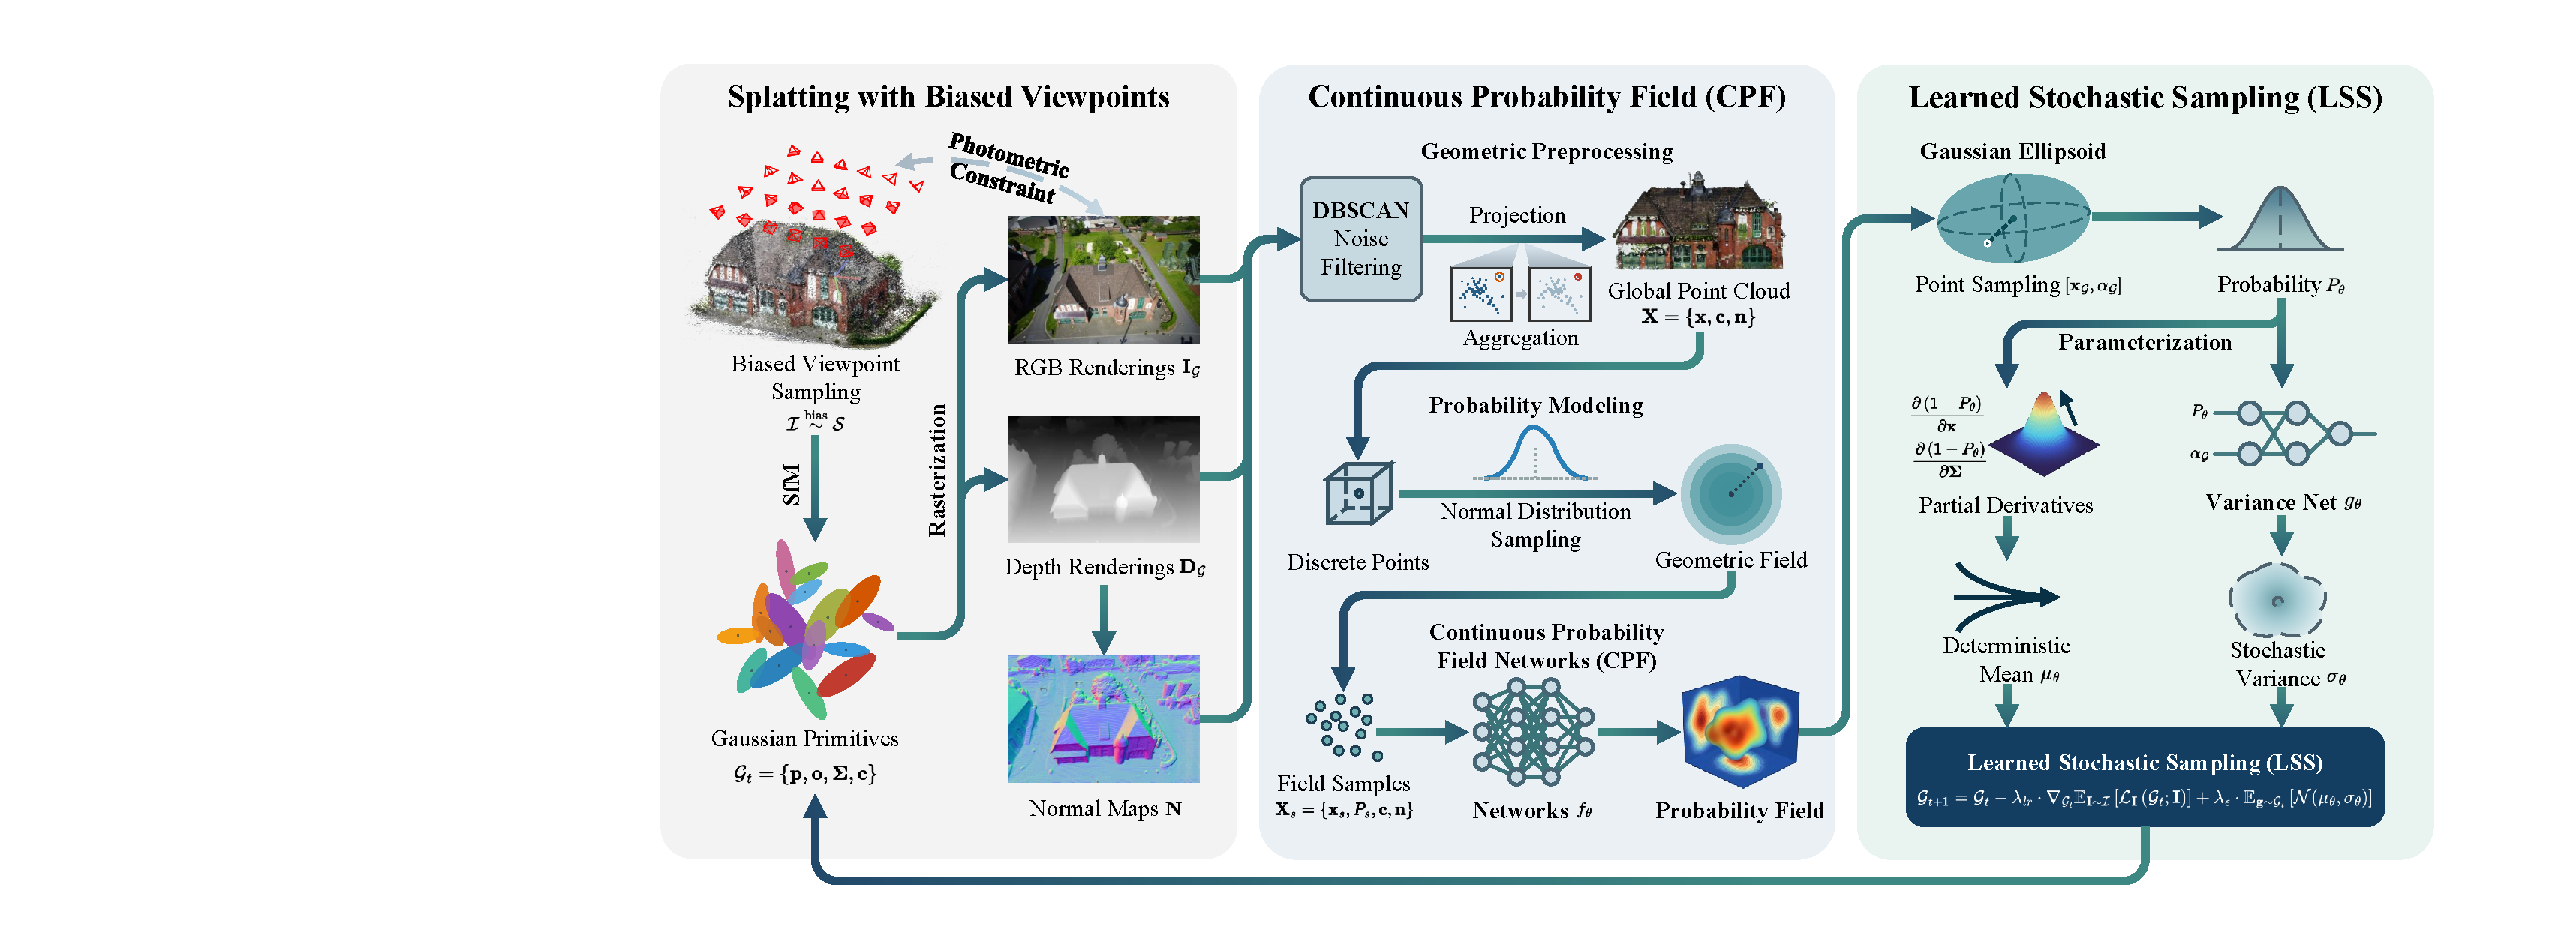
\includegraphics[width=0.99\textwidth]{pics/workflow_new.pdf}
    \caption{The pipeline of our proposed GS-LSS. We optimize Gaussian primitives as a learned stochastic sampling process, where the deterministic and stochastic parameters are learned from the Continuous Probability Field (CPF). The CPF is trained from a probabilized geometry field, which includes points, colors, normals, and corresponding probabilities.}
    \label{fig_2}
\end{figure*}

Our approach addresses the biased observation problem by introducing observed-support regularized Learned Stochastic Sampling. The overall workflow is illustrated in Fig.~\ref{fig_2}.

\subsection{Preliminary}

Let $\mathcal{G} = \{\mathbf{g}_i\}_{i=1}^N$ denote the Gaussian field, $\mathcal{I} = \{\mathbf{I}_j\}_{j=1}^M$ denote the training view distribution where $\mathbf{I}_j$ is the $j$-th training view, $\mathcal{S}$ denote the reliable scene support, and $\mathcal{P}(\mathcal{G} \vert \mathcal{S})$ denote the posterior distribution of the Gaussian field given the $\mathcal{S}$. 

3DGS-MCMC~\cite{mcmc} reformulates Gaussian updates as a stochastic optimization process. Its update can be written in a Langevin Monte Carlo (LMC)~\cite{sgld} form as follows:
\begin{equation}
    \mathcal{G}_{t+1} = \mathcal{G}_t + \alpha \cdot \nabla_{\mathcal{G}_t} \log \mathcal{P}(\mathcal{G}_t \vert \mathcal{S}) + \beta \cdot \epsilon_{\mathcal{G}_t \vert \mathcal{S}}, 
    \label{eq1}
\end{equation}
where the gradient term provides a deterministic drift and $\epsilon_{\mathcal{G}_t \vert \mathcal{S}}$ enables stochastic exploration to escape local minima.

In practice, 3DGS-MCMC~\cite{mcmc} approximates this update primarily through the photometric loss, which is reliable only when the viewpoint distribution $\mathcal{I}$ sufficiently covers the scene support.
\begin{equation}
    \mathcal{P}(\mathcal{G} \vert \mathcal{S}) \propto \exp \left( - \mathcal{L}_{\mathbf{I}} \right), 
    \label{eq2}
\end{equation}
\begin{equation}
    \mathcal{L}_{\mathbf{I}} = \left( 1 - \eta_{\mathbf{I}} \right) \cdot \mathcal{L}_{1} + \eta_{\mathbf{I}} \cdot \mathcal{L}_{ssim} + \eta_{o} \cdot \vert o \vert + \eta_{\mathbf{\Sigma}} \vert \sqrt{\text{eig}(\mathbf{\Sigma})} \vert, 
    \label{eq3}
\end{equation}
where $\mathbf{I} \sim \mathcal{I}$ are the training views; $\mathcal{L}_{\mathbf{I}}$ is the pixel-wise loss function; $\text{eig}(\cdot)$ denotes the eigenvalues of the covariance matrix; $\eta$ terms are hyperparameters.
The stochastic perturbation $\sigma_{mc}$, which samples around the photometric gradients, is defined exclusively on the locations of the Gaussians with 
\begin{equation}
    \sigma_{mc} = \frac{\lambda_{lr} \cdot \mathbf{\Sigma}}{1 + e^{100 \cdot \left( 0.995 - \mathbf{o} \right)}}.
    \label{eq4}
\end{equation}

Although 3DGS-MCMC~\cite{mcmc} improves the robustness of view synthesis through stochastic optimization, its practical update is still dominated by photometric gradients, and its hand-crafted stochasticity provides only limited exploration around the optimization bias. 
Therefore, we approximate an aggregated observed-support field and use it to regularize the stochastic Gaussian optimization process. 

\subsection{Learned Stochastic Sampling}

\subsubsection{Problem Statement}

The key assumption behind the 3DGS-MCMC~\cite{mcmc} stochastic optimization is that the viewpoint distribution $\mathcal{I}$ sufficiently covers the reliable scene support $\mathcal{S}$. However, in biased viewpoint scenarios, the training observations represent a severely \emph{biased sampling} of the ideal scene support,
\begin{equation}
    \mathcal{I}_{\text{bias}} \neq \mathcal{I}_{\text{ideal}} \sim \mathcal{S}.
    \label{eq5}
\end{equation}
where $\mathcal{I}_{\text{bias}}$ and $\mathcal{I}_{\text{ideal}}$ denote the biased and ideal viewpoint distributions, respectively.
As a result, minimizing the photometric loss alone from biased samples cannot enforce reliable scene consistency. We refer to this phenomenon as \emph{perspective overfitting}. One way to quantify this mismatch is the gap $\Delta_{\text{overfit}}$ between the expected loss under ideal and biased viewpoint distributions,
\begin{equation}
    \Delta_{\text{overfit}} = \mathbb{E}_{\mathbf{I} \sim \mathcal{I}_{\text{ideal}}} \left[ \mathcal{L}_{\mathbf{I}} (\mathcal{G}; \mathbf{I}) \right] - \mathbb{E}_{\mathbf{I} \sim \mathcal{I}_{\text{bias}}} \left[ \mathcal{L}_{\mathbf{I}} (\mathcal{G}; \mathbf{I}) \right],
    \label{eq5.1}
\end{equation}
where $\vert \Delta_{\text{overfit}} \vert$ is a conceptual measure expected to grow with the bias severity of the viewpoint coverage, so the photometric gradients derived from severely biased observations can become poorly aligned with reliable scene support.

Addressing this challenge requires a direct constraint that regularizes the Gaussian field $\mathcal{G}$ toward reliable observed support, without assuming that fully unobserved structure can be recovered from biased views.
Therefore, we define the following observed-support regularized surrogate objective,
\begin{equation}
    \pi^{\star} (\mathcal{G}) \propto \exp \left( - \mathbb{E}_{\mathbf{I}\sim\mathcal{I}_{\text{bias}}}\!\left[\mathcal{L}_{\mathbf{I}}(\mathcal{G};\mathbf{I})\right] - \lambda_{s} \mathcal{R}(\mathcal{G};\mathcal{S}) \right),
    \label{eq6.5}
\end{equation}
where $\mathcal{R}(\cdot)$ is a one-sided observed-support penalty and $\lambda_{s}$ balances the photometric loss and the support regularization. Eq.~\ref{eq6.5} should be understood as a practical optimization objective rather than a claim that the full scene support is exactly recovered.

\subsubsection{Parameterization of \texorpdfstring{$\mu_{\theta}$}{mu-theta}}

Assuming an ideal support field $\mathcal{S}$ is given, we then rewrite the corresponding surrogate energy as, 
\begin{equation}
    -\log \pi^{\star} (\mathcal{G}) \triangleq \underbrace{\mathbb{E}_{\mathbf{I}\sim\mathcal{I}}\!\left[\mathcal{L}_{\mathbf{I}}(\mathcal{G};\mathbf{I})\right]}_{\text{view-dependent}}
    + \lambda_{s} \underbrace{\mathcal{R}(\mathcal{G};\mathcal{S})}_{\text{observed-support reg}} + C,
    \label{eq7}
\end{equation}
where $C$ is a constant independent of $\mathcal{G}$. The view-dependent term preserves faithfulness to the training views, while the support term regularizes the Gaussian field toward reliable observed support. Substituting Eq.~\ref{eq7} into Eq.~\ref{eq1} gives, 
\begin{equation}
    \begin{aligned}
    \mathcal{G}_{t+1} = &\mathcal{G}_t - \alpha \cdot \nabla_{\mathcal{G}_t} \mathbb{E}_{\mathbf{I}\sim\mathcal{I}_{\text{bias}}}\!\left[\mathcal{L}_{\mathbf{I}}(\mathcal{G}_t;\mathbf{I})\right] \\
    &- \alpha \lambda_s \cdot \nabla_{\mathcal{G}_t} \mathcal{R}(\mathcal{G}_t;\mathcal{S}) + \beta \cdot \epsilon_{\mathcal{G}_t \vert \mathcal{S}}.
    \end{aligned}
    \label{eq8}
\end{equation} 

To regularize the Gaussian field $\mathcal{G}$ with the support field $\mathcal{S}$, we define the one-sided observed-support penalty $\mathcal{R}(\cdot)$ as the expectation over Gaussian primitives, 
\begin{equation}
    \mathcal{R}(\mathcal{G};\mathcal{S}) = \mathbb{E}_{\mathbf{g} \sim \mathcal{G}} \left[ \mathbf{1} - \mathcal{S} (\mathbf{g}) \right],
    \label{eq9}
\end{equation}
where $\mathcal{S} (\mathbf{g}) \in [0, 1]$ denotes the ideal support probability, i.e., the compatibility of Gaussian $\mathbf{g}$ with reliable scene support.

In practice, $\mathcal{S}$ is often unavailable under biased viewpoints. Therefore, we use a neural network to estimate an observed support surrogate from in-training geometric priors. We name this model Continuous Probability Field (CPF), denoted $f_{\theta}$, 
\begin{equation}
    \mathcal{S}(\mathbf{g}) \approx f_{\theta}(\mathbf{g}), 
    \label{eq10}
\end{equation}
where $f_{\theta}(\mathbf{g})$ predicts the probability of a given 3D primitive being supported by the aggregated observed scene structure. 
A larger deviation of the Gaussian primitive from this observed support corresponds to a lower probability.

Now, we can obtain a tractable observed-support penalty:
\begin{equation}
    \widehat{\mathcal{R}}(\mathcal{G};\mathcal{S}) = \mathbb{E}_{\mathbf{g} \sim \mathcal{G}} \left[ 1 - f_{\theta} (\mathbf{g}) \right].
    \label{eq11}
\end{equation}
Let $\delta(\mathbf{g})= f_{\theta} (\mathbf{g}) - \mathcal{S} (\mathbf{g})$ denote the CPF approximation error. Then, we have
\begin{equation}
    \begin{aligned}
    \nabla_{\mathcal{G}_t} \widehat{\mathcal{R}}(\mathcal{G}_t;\mathcal{S}) - \nabla_{\mathcal{G}_t} \mathcal{R}(\mathcal{G}_t;\mathcal{S}) &= \nabla_{\mathcal{G}_t} \mathbb{E}_{\mathbf{g} \sim \mathcal{G}_t} \left[ \delta(\mathbf{g}) \right], \\
    % \delta(\mathbf{g}) &= f_{\theta} (\mathbf{g}) - \mathcal{S} (\mathbf{g}).
    \end{aligned}
    \label{eq12}
\end{equation}
This term measures the local sensitivity of the CPF, not a convergence guarantee. Replacing the ideal support $\mathcal{S}$ with CPF changes the support gradient direction by the residual drift in Eq.~\ref{eq12}. When the aggregated priors are reliable, the drift can be reduced and the CPF mainly stabilizes weakly observed Gaussians. The global aggregation, delayed start, normal smoothness, DBSCAN filtering, and observation-aware gating in Section~\ref{sec:cpf} are therefore safeguards that reduce, but do not eliminate, CPF error.

By replacing $\mathcal{R}(\cdot)$ with $\widehat{\mathcal{R}}(\cdot)$ in Eq.~\ref{eq8}, we have, 
\begin{equation}
    \begin{aligned}
    \mathcal{G}_{t+1} = &\mathcal{G}_t - \alpha \cdot \nabla_{\mathcal{G}_t} \mathbb{E}_{\mathbf{I}\sim\mathcal{I}_{\text{bias}}}\!\left[\mathcal{L}_{\mathbf{I}}(\mathcal{G}_t;\mathbf{I})\right] \\
    &- \alpha \lambda_s \cdot \nabla_{\mathcal{G}_t} \mathbb{E}_{\mathbf{g} \sim \mathcal{G}_t} \left[ 1 - f_{\theta}( \mathbf{g} ) \right] + \beta \cdot \epsilon_{\mathcal{G}_t \vert \mathcal{S}}.
    \end{aligned}
    \label{eq13}
\end{equation}
Therefore, the learned deterministic drift is defined as, 
\begin{equation}
    \mu_{\theta} = -  \nabla_{\mathbf{g}}  (1 - f_{\theta}(\mathbf{g})).
    \label{eq13.1}
\end{equation}
The parameterization of $\mu_{\theta}$ provides explicit observed-support guidance for the Gaussians by regularizing them toward the observed-support field.

\subsubsection{Parameterization of \texorpdfstring{$\sigma_{\theta}$}{sigma-theta}}

The stochasticity of the LMC sampling process is crucial for global exploration. 
Under biased viewpoints, a good perturbation should depend on both the observed support field and the current Gaussian states. 
In addition, as discussed in~\cite{sgld2}, the variance should be adaptive to the training state. Therefore, we propose to parameterize $\epsilon_{\mathcal{G}_t \vert \mathcal{S}}$ with a variance network $g_{\theta}$ that takes the predicted probability from $f_{\theta}$ and the Gaussian field $\mathcal{G}_t$ as input,
\begin{equation}
    \epsilon_{\mathcal{G}_t \vert \mathcal{S}} = \mathcal{N} (0, \sigma_{\theta}), \sigma_{\theta} = g_{\theta}\big(f_{\theta}(\mathcal{G}_t); \mathcal{G}_t\big).
    \label{eq15}
\end{equation}
Compared with the hand-crafted stochasticity in 3DGS-MCMC~\cite{mcmc}, the parameterization of $\sigma_{\theta}$ is conditioned on both the observed support field and the Gaussian states. When Gaussian primitives are far from the observed support, the low probability predicted by the CPF model yields a large variance, encouraging stronger exploration to escape local minima.

\subsubsection{Final Formulation}

Combining Eq.~\ref{eq13.1} and Eq.~\ref{eq15}, we implement GS-LSS as a per-primitive reparameterized stochastic update. For primitive $i$, let $\boldsymbol{\tau}_i=[\mathbf{p}_i,\boldsymbol{\rho}_i,\mathbf{q}_i]$ denote the center, log-scale, and normalized-rotation parameters defined in Sec.~\ref{sec:cpf}. The update is
\begin{align}
    \boldsymbol{\tau}_i^{t+1}
    &= \boldsymbol{\tau}_i^{t}
    - \lambda_{lr}\nabla_{\boldsymbol{\tau}_i}\mathcal{L}_{\mathbf{I}}
    + \lambda_s \mu_{\theta,i} \notag\\
    &\quad
    + \lambda_{\epsilon}\sigma_{\theta,i}\odot\boldsymbol{\xi}_i,
    \quad \boldsymbol{\xi}_i\sim\mathcal{N}(0,\mathbf{I}), \label{eq16}\\
    \mu_{\theta,i} &= \nabla_{\boldsymbol{\tau}_i} f_{\theta}(\mathbf{x}_{\mathcal{G},i}), \label{eq17}\\
    \sigma_{\theta,i} &=
    g_{\theta}\big(f_{\theta}(\mathbf{x}_{\mathcal{G},i}),\alpha_{\mathcal{G},i}; \boldsymbol{\tau}_i\big). \label{eq18}
\end{align}
This form makes the role of $\sigma_{\theta,i}$ explicit: it scales the sampled noise rather than disappearing inside an expectation. We use the stochastic formulation as a learned optimizer rather than an exact Langevin or Metropolis-Hastings sampler, and therefore do not claim a stationary sampling distribution.

The effectiveness of $\mu_{\theta}$ and $\sigma_{\theta}$ depends on the accuracy of the observed support approximation by the CPF model. Therefore, the training priors and loss functions for the CPF model are crucial for the performance of our LSS method.

\subsection{Continuous Probability Field}\label{sec:cpf}

The target of the CPF model $f_{\theta}$ is to provide 
a data-driven approximation of the aggregated observed-support field $\mathcal{S}(\mathbf{g})$ (Eq.~\ref{eq10}).
{Operationally, the CPF probability $P_{\theta}$ is queried at points sampled from Gaussian primitives, which denotes observed-support probability rather than a posterior over unseen geometry.}
The accuracy of the CPF model is reflected in the residual drift in Eq.~\ref{eq12}.
To construct this approximation from biased training samples, we supervise $f_{\theta}$ with an in-training probabilized geometry field aggregated from all training views.

The geometry that supervises the CPF model is itself derived from 3DGS under biased viewpoints, so the CPF model is not claimed to recover fully unobserved geometry. Instead, it estimates a smooth observed-support field from evidence aggregated across all available training views, and uses this field to regularize updates only where per-view supervision is under-determined. In our training schedule, CPF supervision starts after the initial Gaussian field has stabilized, and learned LSS sampling is enabled only after the CPF has received its first supervision stage. The global aggregation, DBSCAN outlier filtering, normal-driven smoothness, and observation-aware gating reduce the risk that a single biased view dominates the field.


\subsubsection{In-training Geometric Field}

Given Gaussian ellipsoids 
$\mathcal{G}_t = \{\mathbf{g}_i\}_{i=1}^N$, where $\mathbf{g}_i = \{ \mathbf{p}, \mathbf{o}, \mathbf{\Sigma}, \mathbf{c} \}$ 
at training iteration $t$, we first render RGB images $\mathbf{I}_{\mathcal{G}}$ and depth maps $\mathbf{D}_{\mathcal{G}}$ from the training views, and compute the normal maps $\mathbf{N}$ from the depth maps. 
After DBSCAN outlier filtering, 
we project these maps and aggregate them into the world coordinate system to construct a global sparse point cloud $\mathbf{X} = \{ \mathbf{x}, \mathbf{c}, \mathbf{n} \}$, where $\mathbf{x}$ is the 3D coordinate, $\mathbf{c}$ is color, and $\mathbf{n}$ is normal.

To obtain probabilistic supervision without making the field dependent on the absolute scene scale, we first normalize the scene coordinates by the scene center $\mathbf{c}_{\mathrm{sc}}$ and diagonal length $d_{\mathrm{sc}}$, i.e., $\tilde{\mathbf{x}}=(\mathbf{x}-\mathbf{c}_{\mathrm{sc}})/d_{\mathrm{sc}}$. We then sample around each normalized point and compute its probability,
\begin{align}
    \tilde{\mathbf{x}}_{s} &\sim \mathcal{N}(\tilde{\mathbf{x}}, \sigma_s^2\mathbf{I}_3), \label{eq19} \\
    P_{s} &= \exp\left(-\frac{\|\tilde{\mathbf{x}}_{s}-\tilde{\mathbf{x}}\|_2^2}{2\sigma_s^2}\right), \label{eq20}
\end{align}
where $\sigma_s$ is set proportional to the median nearest-neighbor distance of the aggregated point cloud in normalized coordinates. We thus acquire the geometry field $\mathbf{X}_{s} = \{ \tilde{\mathbf{x}}_{s}, P_{s}, \mathbf{c}, \mathbf{n} \}$ as the training priors. This normalization makes the CPF supervision comparable across datasets with different physical scales.

\subsubsection{CPF network and Loss Function}

We build the CPF network $f_{\theta}$ with a 3-layer SIREN~\cite{implicit}-style MLP, which maps sampled points $\mathbf{x}_{s}$ to the probability $P_{\theta}$ and color $\mathbf{c}_{\theta}$.
During training, the depth normals are consistently oriented before aggregation, and the normalized CPF gradient $\hat{\mathbf{n}}_{\theta}=\nabla_{\mathbf{x}}P_{\theta}/(\|\nabla_{\mathbf{x}}P_{\theta}\|_2+\epsilon_n)$ is regularized by $\mathbf{n}$ to encourage field continuity and smoothness. The loss function is defined as:
\begin{equation}
    \begin{aligned}
    \mathcal{L}_{cpf} = &\sum_{\mathbf{x}} \vert P_{\theta} - P_{s} \vert + \sum_{\mathbf{x}}  \vert 1 - \langle\mathbf{n}, \nabla_{\mathbf{x}} P_{\theta}\rangle \vert \\
    &+ \sum_{\mathbf{x}} \vert \mathbf{c}_{\theta} - \mathbf{c} \vert
    \end{aligned}
    \label{eq21}
\end{equation}
where $\langle\cdot,\cdot\rangle$ denotes cosine similarity. Fig.~\ref{fig_3} shows an example of the trained CPF model.

\begin{figure}[!t]
    \centering
    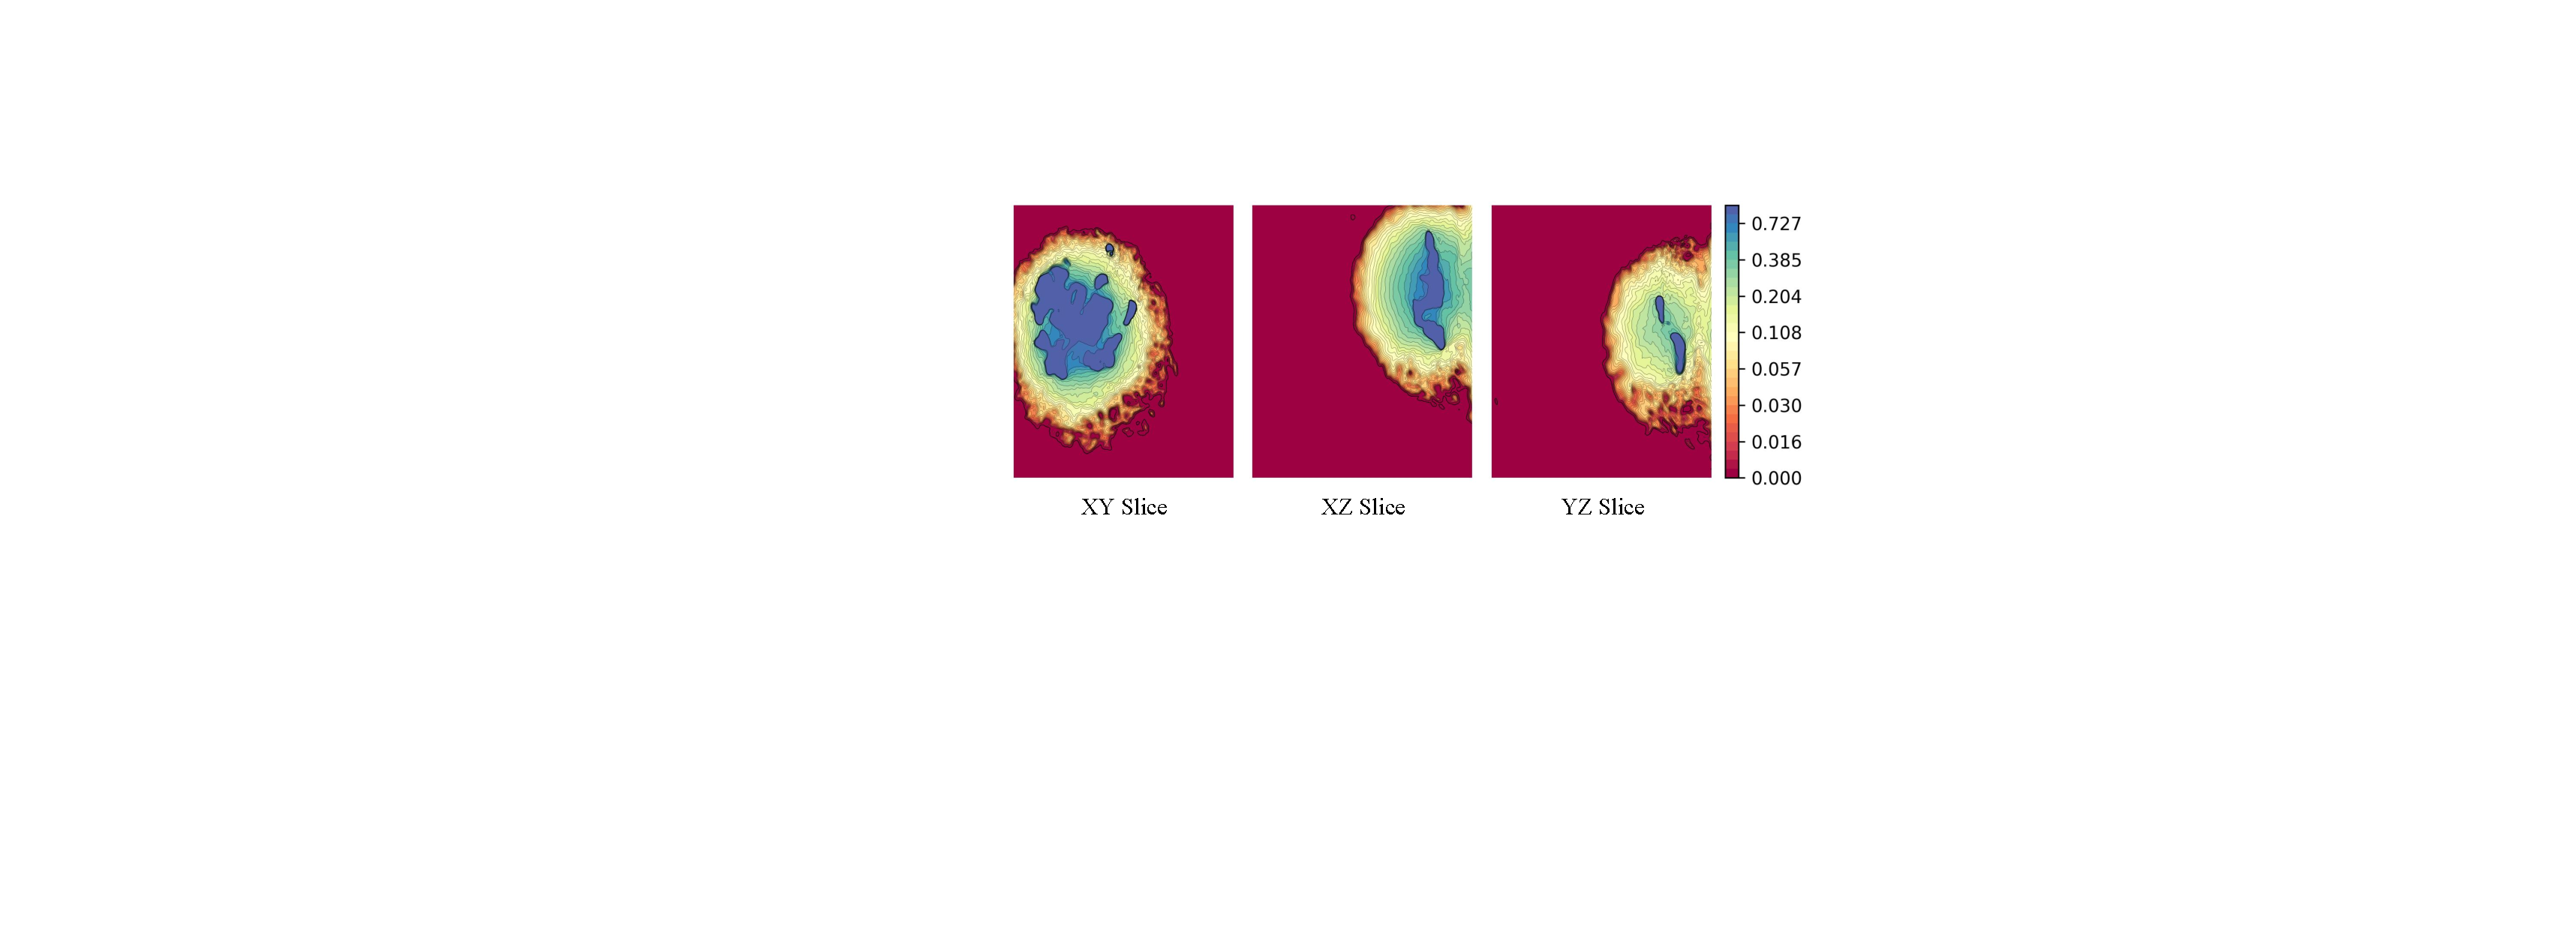
\includegraphics[width=0.49\textwidth]{pics/cpf.pdf}
    \caption{A visual example of a trained Continuous Probability Field (CPF). The panels show $x-y$, $x-z$, and $y-z$ slices, {\color{blue}blue} and {\color{red}{red}} denote high and low observed-support probability, respectively.}
    \label{fig_3}
\end{figure}

Since the loss function is built upon globally aggregated geometric priors, it encourages the CPF network $f_{\theta}$ to behave as an observed-support estimator rather than a per-view regressor, which is designed to reduce the residual drift $\nabla_{\mathcal{G}_t} \mathbb{E}_{\mathbf{g} \sim \mathcal{G}_t} \left[ \delta(\mathbf{g}) \right]$ in Eq.~\ref{eq12} when the priors are reliable. This is the practical distinction from regularization-based methods, whose regularization is derived from per-view perspectives.

\subsubsection{Computation of \texorpdfstring{$\mu_{\theta}$ and $\sigma_{\theta}$}{mu-theta and sigma-theta}}

To make the LSS update of Eq.~\ref{eq16} concrete, we compute the deterministic drift ${\mu}_{\theta,i}$ and the stochastic scale ${\sigma}_{\theta,i}$ as explicit, differentiable functions of the CPF predictions and the Gaussian states.
Different from 3DGS-MCMC~\cite{mcmc}, we update both the locations and shapes of the Gaussian ellipsoids through the gradients provided by the CPF model. For each Gaussian ellipsoid $\mathbf{g}_i = \{\mathbf{p}_i, \mathbf{o}_i, \mathbf{\Sigma}_i, \mathbf{c}_i\} \sim \mathcal{G}$, we randomly sample a point within it and compute its opacity, 
\begin{align}
    \mathbf{x}_{\mathcal{G},i} &\sim \mathcal{N} \left( \mathbf{p}_i, \mathbf{\Sigma}_i \right), \label{eq22} \\
    \alpha_{\mathcal{G},i} &= e^{-\frac{1}{2} \left( \mathbf{x}_{\mathcal{G},i} - \mathbf{p}_i \right)^{T} \mathbf{\Sigma}_i^{-1} \left( \mathbf{x}_{\mathcal{G},i} - \mathbf{p}_i \right)} \cdot \mathbf{o}_i. \label{eq23}
\end{align}
The CPF then gives the per-Gaussian support probability $P_{\theta,i}=f_{\theta}(\mathbf{x}_{\mathcal{G},i})$.

% These points are fed into the CPF model to obtain the probability $P_{\theta}=f_{\theta}(\mathbf{x}_{\mathcal{G}})$. 
In implementation, we do not directly update the raw covariance matrix. Instead, the covariance is parameterized as $\mathbf{\Sigma}_i=\mathbf{R}(\mathbf{q}_i)\operatorname{diag}(\exp(2\boldsymbol{\rho}_i))\mathbf{R}(\mathbf{q}_i)^{T}$, where $\boldsymbol{\rho}_i$ are log-scales and $\mathbf{q}_i$ is a normalized quaternion. Therefore, the LSS geometry parameter is $\boldsymbol{\tau}_i=[\mathbf{p}_i,\boldsymbol{\rho}_i,\mathbf{q}_i]$, which preserves the positive definiteness of $\mathbf{\Sigma}_i$ during optimization. Following Eq.~\ref{eq17}, the deterministic drift is obtained by back-propagating the CPF probability to these parameters:
\begin{equation}
    {\mu}_{\theta,i}= -\nabla_{\boldsymbol{\tau}_i}(1-P_{\theta,i})=\nabla_{\boldsymbol{\tau}_i}P_{\theta,i}.
    \label{eq24}
\end{equation}
This drift moves each Gaussian toward higher support $P_{\theta,i}$ while keeping the covariance representation valid.

The variance module is implemented with two lightweight 2-layer MLP heads. The scale head $g_{\theta}$ predicts a learnable scale $a_{\theta,i}$, and the gate head $h_{\theta}$ predicts an observation-aware confidence gate $\Delta_{\theta,i}$ from the observed support $P_{\theta,i}$ and sampled opacity $\alpha_{\mathcal{G},i}$:
\begin{equation}
    a_{\theta,i} = g_{\theta}\left(P_{\theta,i}, \alpha_{\mathcal{G},i}\right),\quad 
    \Delta_{\theta,i} = h_{\theta}\left(P_{\theta,i}, \alpha_{\mathcal{G},i}\right),
    \label{eq25.01}    
\end{equation}
\begin{equation}
    {\sigma}_{\theta,i} = \frac{a_{\theta,i} \cdot \mathbf{D}_i}{1 + e^{100 \cdot \Delta_{\theta,i}}}, 
    \label{eq25}
\end{equation}
where $\mathbf{D}_i$ is a diagonal parameter-space scale matrix: its position block uses the current Gaussian axis scales $\exp(\boldsymbol{\rho}_i)$, while the log-scale and rotation blocks use fixed small constants. $P_{\theta}$ measures support from the CPF field, and $\alpha_{\mathcal{G}}$ measures primitive support at the sampled point.
The learned gate suppresses ${\sigma}_{\theta,i}$ for well-observed primitives and allows larger perturbations for weakly supported primitives. The factor 100 follows the sharp confidence gate used in 3DGS-MCMC~\cite{mcmc}. We clamp the exponent for numerical stability. The heads $g_{\theta}$ and $h_{\theta}$ are not trained with a separate variance target. After the one-step reparameterized update in Eq.~\ref{eq16}, Eq.~\ref{eq26} is back-propagated through $\mu_{\theta,i}$ and $\sigma_{\theta,i}$ using first-order gradients, without multi-step unrolling or second-order derivatives. Thus, ${\sigma}_{\theta,i}$ is a train-time perturbation scale rather than a calibrated posterior variance, replacing the hand-crafted opacity rule in Eq.~\ref{eq4} with a learned observation-conditioned gate.

The LSS process is then performed using Eq.~\ref{eq16}, where ${\mu}_{\theta,i}$ serves as an observed-support drift and ${\sigma}_{\theta,i}$ as an adaptive stochastic perturbation.  

\subsection{Training Objectives}

GS-LSS jointly optimizes the Gaussian field $\mathcal{G}$ and the CPF model $f_{\theta}$, details are provided in Algorithm~\ref{alg:gslss}. Following the surrogate objective in Eq.~\ref{eq7}, the Gaussian field is optimized by the observed-support regularized objective,
\begin{equation}
    \mathcal{L}_{\mathcal{G}} = \mathbb{E}_{\mathbf{I} \sim \mathcal{I}_{\text{bias}}} \left[ \mathcal{L}_{\mathbf{I}}(\mathcal{G};\mathbf{I}) \right] + \lambda_{s} \, \widehat{\mathcal{R}}(\mathcal{G};\mathcal{S}),
    \label{eq26}
\end{equation}
which combines the photometric loss $\mathcal{L}_{\mathbf{I}}$ (Eq.~\ref{eq3}) with the observed-support penalty $\widehat{\mathcal{R}}$ (Eq.~\ref{eq11}). The minimization of $\mathcal{L}_{\mathcal{G}}$ is realized through the LSS update in Eq.~\ref{eq16}, where the deterministic drift ${\mu}_{\theta,i}$ decreases the support penalty and the adaptive perturbation ${\sigma}_{\theta,i}$ injects scene-aware stochastic exploration. The CPF networks are optimized by the geometric-field loss $\mathcal{L}_{cpf}$ (Eq.~\ref{eq21}), which fits $f_{\theta}$ to the globally aggregated probability, color and normal priors. 
We optimize the two objectives jointly so that observed-support estimation and Gaussian optimization remain coupled during training.
Importantly, the CPF and stochastic heads are used only during training. Inference is performed with only the optimized Gaussian field $\mathcal{G}$ with standard 3DGS renderer.    


\begin{algorithm}[t]
\caption{CPF-guided stochastic optimization in GS-LSS}
\label{alg:gslss}
\footnotesize
\begin{algorithmic}[1]
\STATE Initialize $\mathcal{G}$ from SfM points and train with $\mathcal{L}_{\mathbf{I}}$.
\FOR{$t=1,\ldots,T$}
    \STATE Render RGB/depth/normal maps from training views.
    \IF{$t\geq T_{\rm CPF}$}
        \STATE Aggregate geometry; apply DBSCAN; update CPF with Eq.~\ref{eq21}.
    \ENDIF
    \STATE Update ordinary 3DGS attributes with the photometric loss.
    \IF{$t\geq T_{\rm LSS}$}
        \STATE Sample $\mathbf{x}_{\mathcal{G},i}$ from LSS selected Gaussian ellipsoids.
        \STATE Query CPF, compute $\mu_{\theta,i}$ by Eq.~\ref{eq24}, compute $\sigma_{\theta,i}$ by Eq.~\ref{eq25}.
        \STATE Sample $\boldsymbol{\xi}_i\sim\mathcal{N}(0,\mathbf{I})$ and update $\boldsymbol{\tau}_i$ with Eq.~\ref{eq16}.
        \STATE Normalize rotations and keep covariance positive definite.
    \ENDIF
\ENDFOR
\STATE Discard CPF, $g_{\theta}$ and $h_{\theta}$ for inference.
\STATE \textbf{return} optimized Gaussian field $\mathcal{G}$.
\end{algorithmic}
\end{algorithm}

\section{Experiments\label{sec:experiments}}
 
\subsection{Implementation Details}


\subsubsection{Datasets}

We evaluate our method on 16 scenes from 5 widely used datasets, including
8 surrounding scenes 
from Mip-NeRF 360~\cite{mipnerf360},
2 outdoor scenes (Truck and Train) from Tanks \& Temples~\cite{tankstemples},
4 large-scale scenes with planar trajectories from Mill 19~\cite{meganerf},
and 2 urban scenes with both aerial and ground views from MatrixCity~\cite{matrixcity} and Zeche~\cite{isprs}.
These datasets cover a wide range of scene types and viewpoint distributions, providing a comprehensive benchmark.

\begin{table*}[t]
\centering
\caption{Evaluation for systematic coverage gaps on Mip-NeRF 360~\cite{mipnerf360} and Tanks \& Temples~\cite{tankstemples}, with angular gaps 20$^\circ$, 40$^\circ$, 60$^\circ$, 80$^\circ$ and 100$^\circ$. Best results are in \textbf{bold} and second-best are \underline{underlined}.}
\label{tab:coverage_gap}
\scriptsize
\setlength{\tabcolsep}{3.0pt}
\resizebox{\textwidth}{!}{%
\begin{tabular}{lccccccccccccccc}
\toprule
\multirow{2}{*}{Method} & \multicolumn{3}{c}{20$^\circ$} & \multicolumn{3}{c}{40$^\circ$} & \multicolumn{3}{c}{60$^\circ$} & \multicolumn{3}{c}{80$^\circ$} & \multicolumn{3}{c}{100$^\circ$} \\
\cmidrule(lr){2-4}\cmidrule(lr){5-7}\cmidrule(lr){8-10}\cmidrule(lr){11-13}\cmidrule(lr){14-16}
 & SSIM$\uparrow$ & PSNR$\uparrow$ & LPIPS$\downarrow$ & SSIM$\uparrow$ & PSNR$\uparrow$ & LPIPS$\downarrow$ & SSIM$\uparrow$ & PSNR$\uparrow$ & LPIPS$\downarrow$ & SSIM$\uparrow$ & PSNR$\uparrow$ & LPIPS$\downarrow$ & SSIM$\uparrow$ & PSNR$\uparrow$ & LPIPS$\downarrow$ \\
\midrule
\multicolumn{16}{c}{\textbf{Mip-NeRF 360}}\\[-2pt]
\midrule
3DGS~\cite{3dgs} & 0.787 & 24.936 & 0.202 & 0.726 & 22.137 & 0.249 & 0.674 & 20.499 & 0.291 & 0.630 & 19.460 & 0.324 & 0.584 & 17.597 & 0.358 \\
Scaffold-GS~\cite{scaffold} & 0.760 & 23.844 & 0.231 & 0.706 & 21.835 & 0.273 & 0.653 & 20.418 & 0.315 & 0.616 & 19.574 & 0.344 & 0.571 & 17.751 & 0.378 \\
Hierarchical-GS~\cite{hierarchical} & 0.787 & 25.044 & 0.203 & 0.725 & 22.314 & 0.250 & 0.671 & 20.611 & 0.291 & 0.624 & 19.339 & 0.326 & 0.581 & 17.463 & 0.359 \\
MVGS~\cite{mvgs} & 0.784 & 24.827 & 0.203 & 0.715 & 22.130 & 0.256 & 0.658 & 20.458 & 0.303 & 0.608 & 19.081 & 0.340 & 0.561 & 17.164 & 0.374 \\
PGSR~\cite{pgsr} & 0.771 & 24.203 & 0.231 & 0.706 & 21.588 & 0.280 & 0.662 & 20.179 & 0.307 & 0.611 & 18.834 & 0.343 & 0.553 & 16.808 & 0.375 \\
3DGS-MCMC~\cite{mcmc} & \underline{0.801} & \underline{25.323} & \underline{0.194} & \underline{0.739} & \underline{22.369} & \underline{0.239} & 0.679 & 20.732 & \underline{0.283} & 0.632 & 19.344 & \underline{0.319} & 0.572 & 17.204 & \underline{0.355} \\
MH-3DGS~\cite{mh3dgs} & 0.784 & 25.122 & 0.224 & 0.728 & 22.365 & 0.265 & \underline{0.683} & \underline{20.855} & 0.300 & \underline{0.650} & \underline{20.008} & 0.328 & \underline{0.608} & \underline{18.352} & 0.360 \\
GS-LSS (Ours) & \textbf{0.808} & \textbf{25.839} & \textbf{0.188} & \textbf{0.752} & \textbf{23.152} & \textbf{0.236} & \textbf{0.708} & \textbf{21.615} & \textbf{0.273} & \textbf{0.667} & \textbf{20.235} & \textbf{0.307} & \textbf{0.631} & \textbf{18.805} & \textbf{0.340} \\
\addlinespace[2pt]
\midrule
\multicolumn{16}{c}{\textbf{Tanks \& Temples}}\\[-2pt]
\midrule
3DGS~\cite{3dgs} & 0.771 & 20.411 & 0.209 & 0.741 & 19.464 & 0.234 & 0.695 & 18.651 & 0.269 & 0.663 & 17.945 & 0.294 & 0.632 & \underline{17.422} & 0.323 \\
Scaffold-GS~\cite{scaffold} & 0.744 & 19.331 & 0.222 & 0.743 & 19.945 & 0.232 & 0.692 & 18.658 & 0.269 & 0.653 & 17.589 & 0.301 & 0.615 & 17.082 & 0.334 \\
Hierarchical-GS~\cite{hierarchical} & 0.766 & 20.418 & 0.208 & 0.743 & 19.640 & 0.229 & 0.694 & 18.728 & 0.267 & 0.657 & 17.811 & 0.296 & 0.630 & 17.226 & 0.321 \\
MVGS~\cite{mvgs} & 0.756 & 20.211 & \underline{0.199} & 0.721 & 19.150 & 0.229 & 0.668 & 18.323 & 0.275 & 0.625 & 17.549 & 0.309 & 0.590 & 16.875 & 0.340 \\
PGSR~\cite{pgsr} & 0.765 & 20.119 & 0.234 & 0.737 & 19.182 & 0.258 & 0.687 & 18.020 & 0.295 & 0.653 & 17.305 & 0.313 & \underline{0.634} & 17.206 & 0.338 \\
3DGS-MCMC~\cite{mcmc} & \underline{0.782} & \underline{21.026} & 0.202 & \underline{0.754} & \underline{20.018} & \underline{0.220} & \underline{0.702} & \underline{18.973} & \underline{0.257} & \underline{0.665} & \underline{18.014} & \underline{0.285} & 0.632 & 17.406 & \underline{0.317} \\
MH-3DGS~\cite{mh3dgs} & 0.754 & 19.967 & 0.221 & 0.726 & 19.205 & 0.241 & 0.649 & 17.404 & 0.291 & 0.652 & 17.299 & 0.298 & 0.612 & 16.627 & 0.331 \\
GS-LSS (Ours) & \textbf{0.787} & \textbf{21.451} & \textbf{0.191} & \textbf{0.757} & \textbf{20.253} & \textbf{0.210} & \textbf{0.709} & \textbf{19.345} & \textbf{0.247} & \textbf{0.672} & \textbf{18.113} & \textbf{0.274} & \textbf{0.643} & \textbf{17.818} & \textbf{0.304} \\
\bottomrule
\end{tabular}%
}
\end{table*}



\begin{figure*}[t]
    \centering
    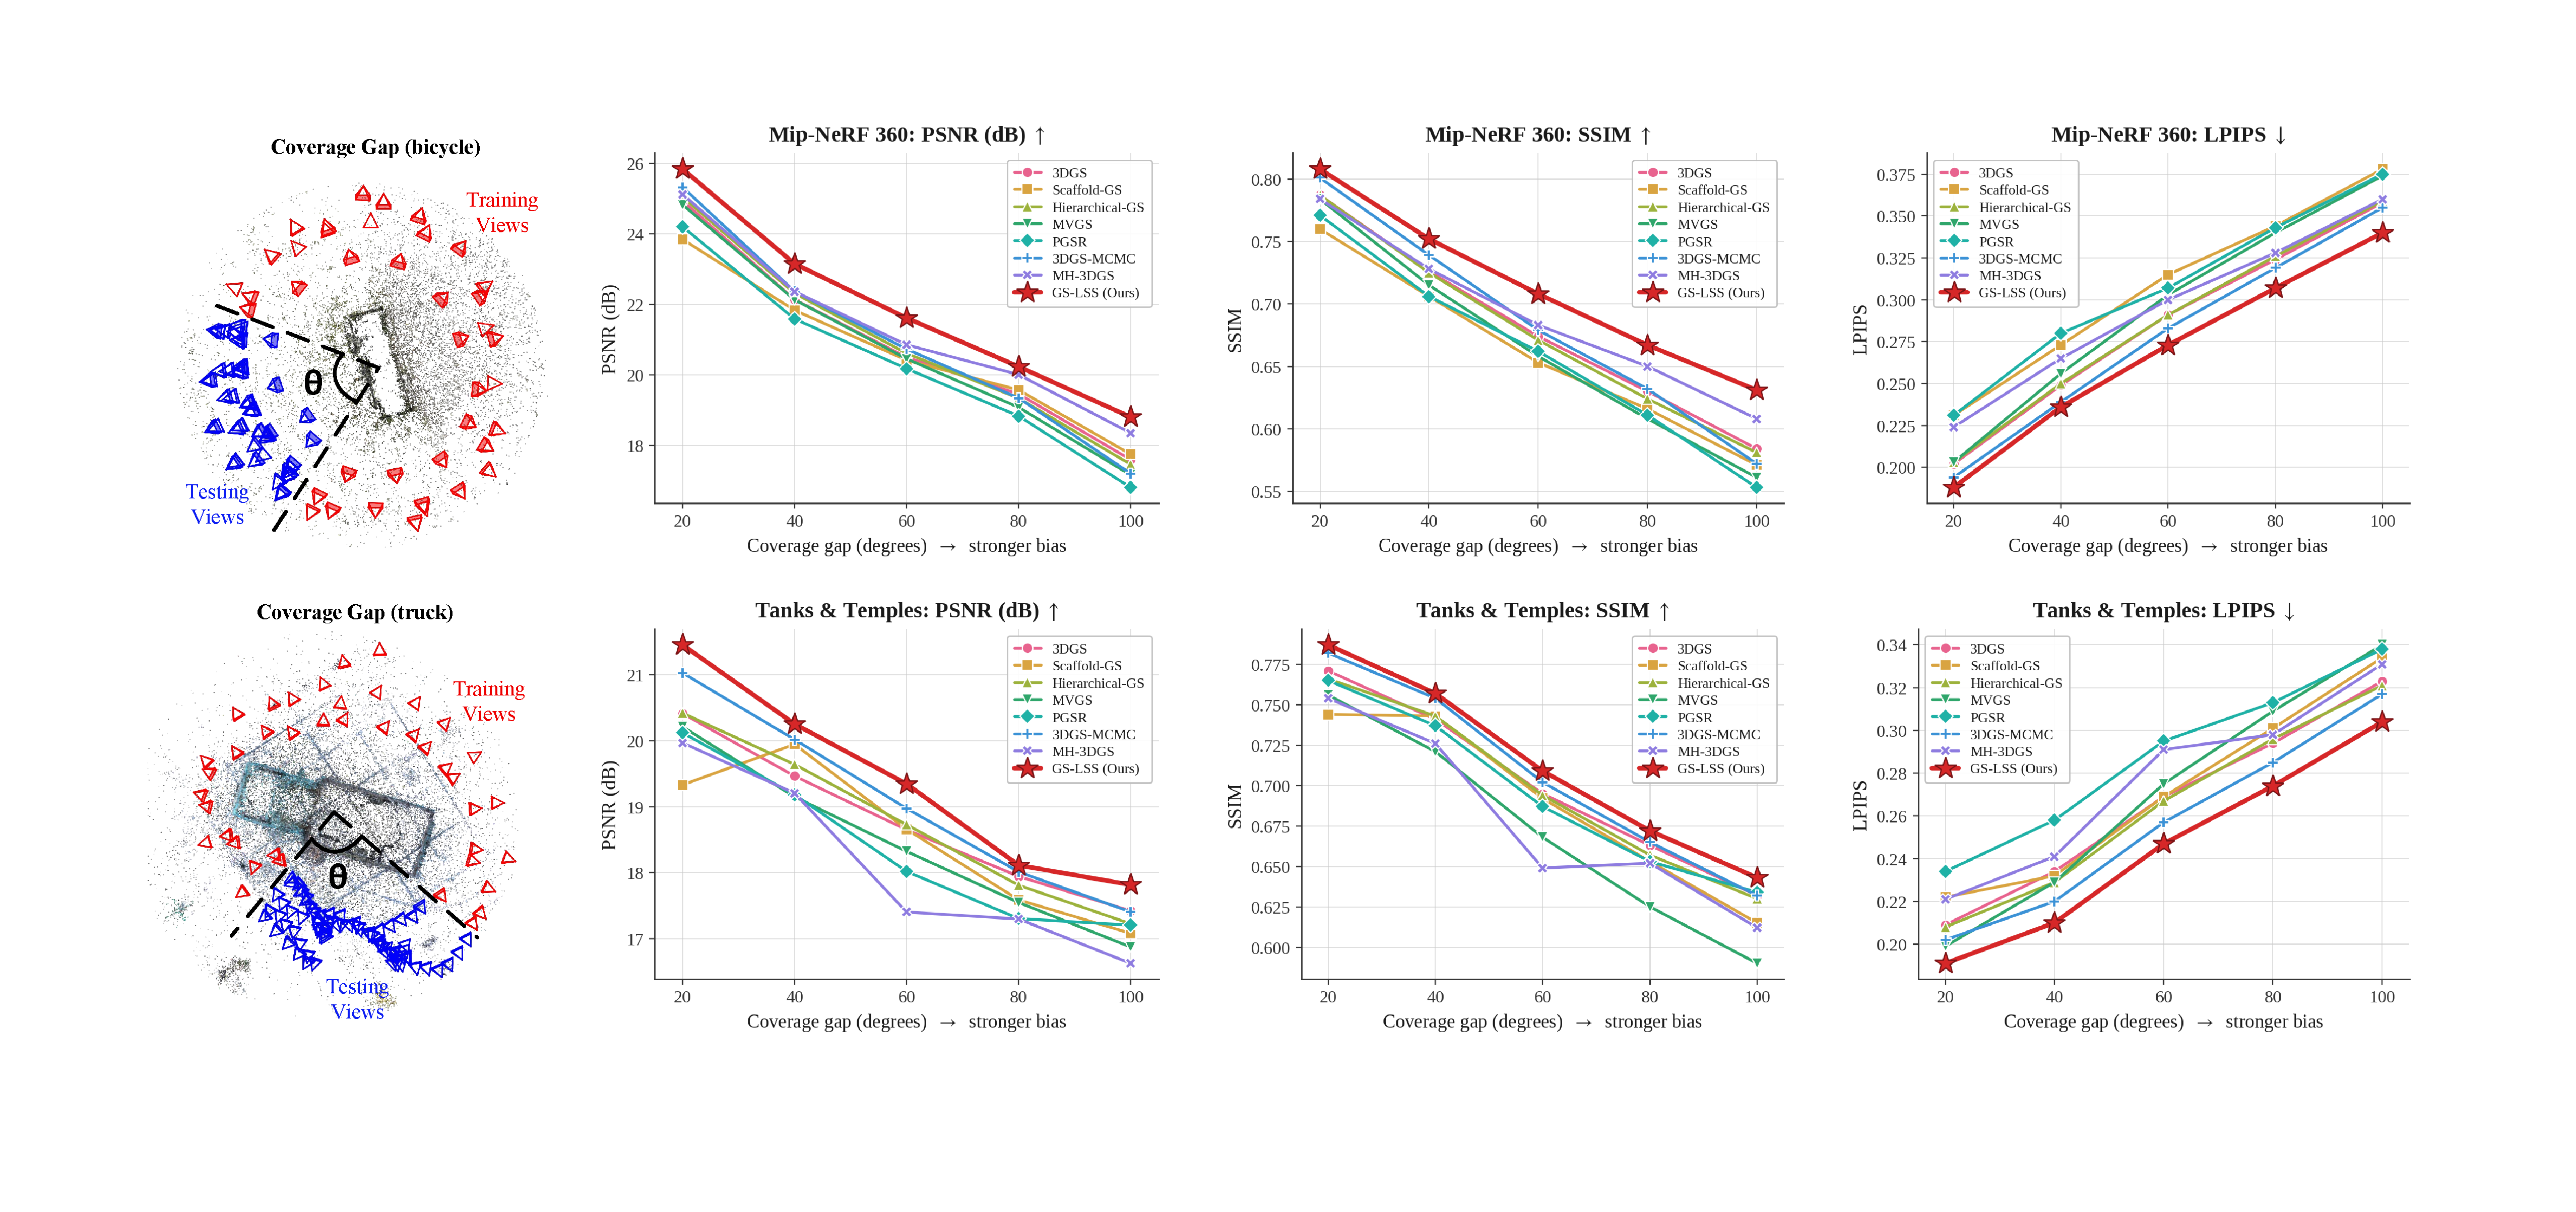
\includegraphics[width=0.95\textwidth]{pics/coverage_gap.pdf}
    \caption{Visualization of the performance trends under systematic coverage gaps, with gap size ranging from 20$^\circ$ to 100$^\circ$. 
    The first row corresponds to Mip-NeRF 360~\cite{mipnerf360} dataset and the second row corresponds to Tanks \& Temples~\cite{tankstemples} dataset.}
    \label{coverage_gap_trend}
\end{figure*}




\subsubsection{Biased Viewpoint Settings}

To evaluate the robustness of our method under various biased viewpoint scenarios, we design three representative settings: \emph{systematic coverage gap}, \emph{discontinuous trajectory} and \emph{viewing angle disparities}.

\textbf{Systematic coverage gap.}
On Mip-NeRF 360~\cite{mipnerf360} and Tanks \& Temples~\cite{tankstemples}, we randomly remove consecutive segments of training views to create angular coverage gaps, where the removed viewpoints are used for evaluation. 
The size of the angular gap is set to a range from 20$^\circ$ to 100$^\circ$ to simulate different severities of systematic coverage gaps.

\textbf{Discontinuous trajectory.}
We evaluate this setting on both surrounding and planar camera trajectories using Mip-NeRF 360~\cite{mipnerf360}, Tanks \& Temples~\cite{tankstemples} and Mill 19~\cite{meganerf}. Specifically, we randomly select several disjoint regions of the viewpoint coverage to form unevenly distributed training views, where each region contains a local cluster of neighboring viewpoints.

\textbf{Viewing angle disparities.}
For this setting, we use Block A of MatrixCity~\cite{matrixcity} and Zeche~\cite{isprs}, as they both contain substantial collections of aerial and ground views. In our experiments, all methods are trained exclusively on aerial views and evaluated on ground views to assess robustness against large view angle disparities.
For all settings, the train/test split is applied before SfM-based initialization. The sparse points for Gaussian initialization, the footprint in Fig.~\ref{perspective_overfitting}, and the FFR support in Table~\ref{tab:ffr} are computed from the selected training views only. No held-out views are used by any method during training or support construction.


\subsubsection{Competitors and Hyperparameters}

We compare our method against representative 3DGS baselines from three families. 
Among them, 3DGS~\cite{3dgs} and Scaffold-GS~\cite{scaffold} are two widely used photometric optimization baselines.
Hierarchical-GS~\cite{hierarchical}, MVGS~\cite{mvgs} and PGSR~\cite{pgsr} are three representative geometric regularization methods for 3DGS.
3DGS-MCMC~\cite{mcmc} and MH-3DGS~\cite{mh3dgs} are two state-of-the-art stochastic optimization baselines.
Particularly, for Hierarchical-GS~\cite{hierarchical}, we enable only depth regularization to ensure a fair comparison.
Methods that require explicit control over the number of Gaussian primitives use the same total count across all competitors. 

All baselines are trained with their official implementations and default configurations under the same training iteration budget, image resolution, fixed train/test split, and the same initialization point cloud. 
Scaffold-GS uses its official anchor and view-adaptive rendering settings.
For our method, CPF training begins at iteration 2000 with a learning rate of $1\times10^{-4}$, 
and the learned sampling of $\mu_{\theta}$ and $\sigma_{\theta}$ begins at iteration 2500.
Unless otherwise stated, the photometric loss of GS-LSS is computed from one randomly sampled training view per iteration, following the standard 3DGS-MCMC~\cite{mcmc} protocol.
Other hyperparameters are set as follows: CPF net $f_{\theta}$ is a 3-layer SIREN-style MLP, $g_{\theta}$ and $h_{\theta}$ are 2-layer MLPs; DBSCAN $\epsilon=0.25$ in normalized coordinates; $\lambda_s=0.1$; and $\lambda_{\epsilon}=1$.
All experiments are conducted on a single NVIDIA RTX 4090 GPU with 24\,GB memory.

\begin{figure*}[!t]
    \centering
    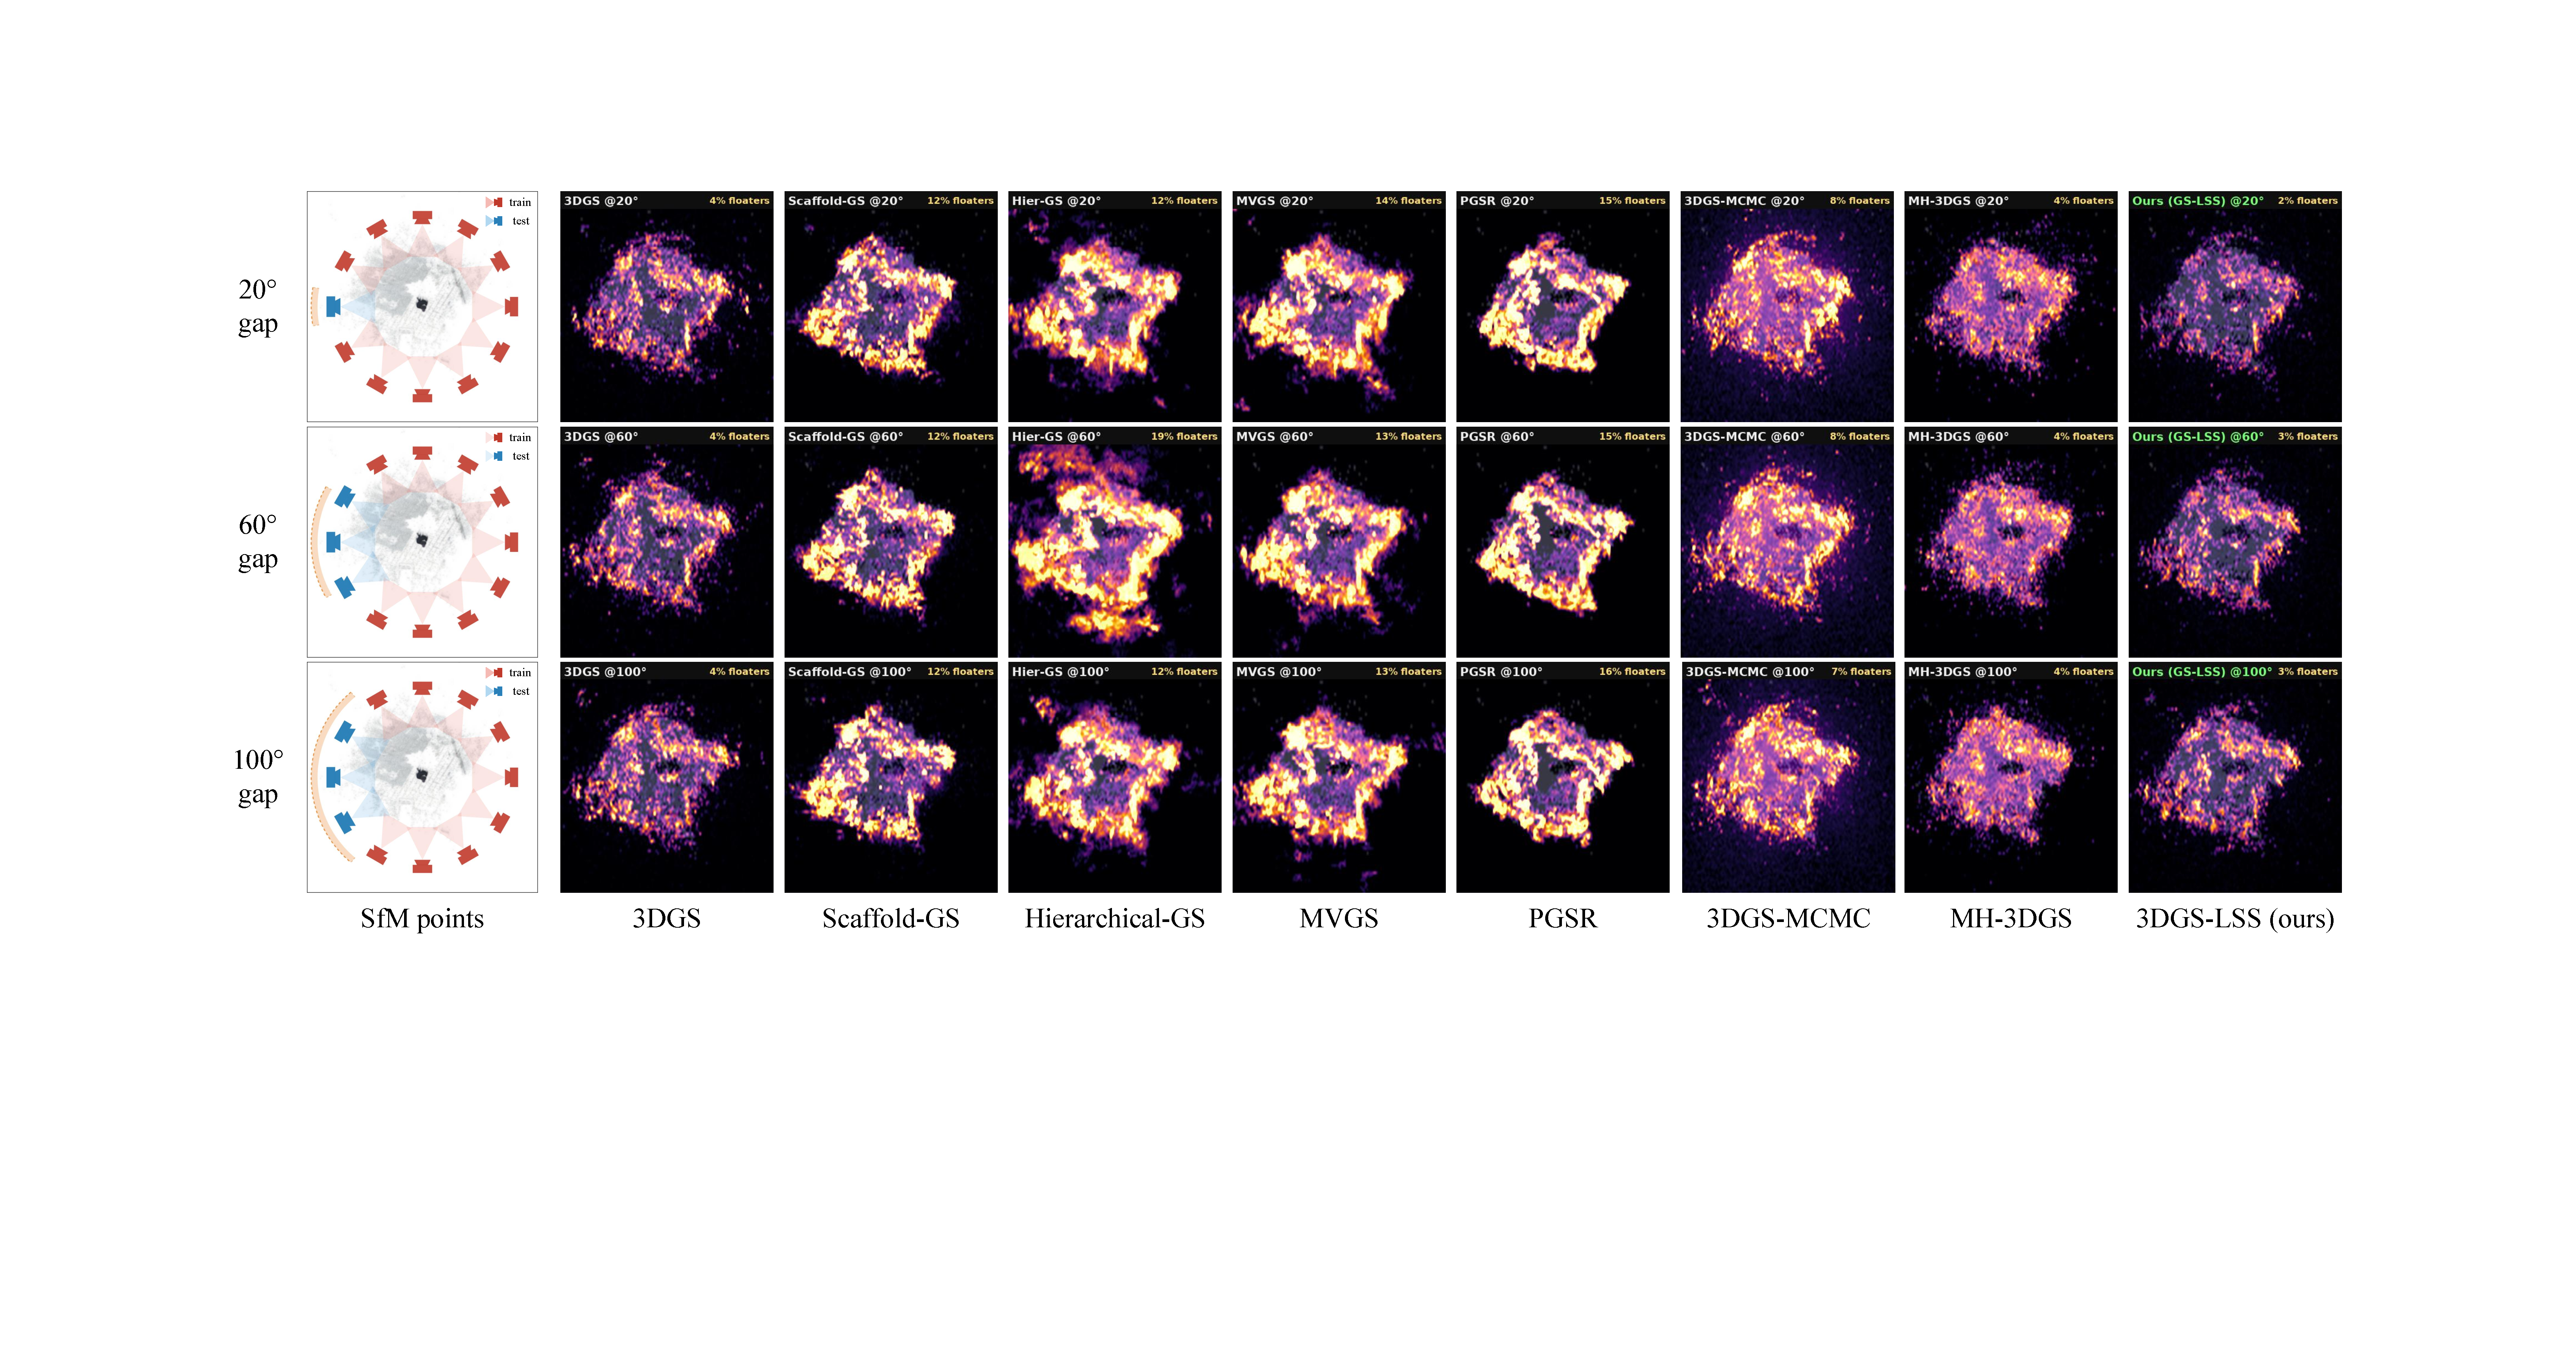
\includegraphics[width=0.97\textwidth]{pics/floters.pdf}
    \caption{Top-down bird's eye view of free-space floaters for the Bonsai scene in Mip-NeRF 360~\cite{mipnerf360} under different systematic coverage gap settings.
    The faint gray shows the SfM footprint, and the hot color map shows the relative density of Gaussians identified as free-space floaters by the visualization protocol.
    }
    \label{perspective_overfitting}
\end{figure*}




\subsection{Main Results}


We organize the experiments to test our core claims: 
1) performance degradation under biased viewpoints is consistent with perspective overfitting.
2) hand-crafted stochastic exploration alleviates this issue, but remains limited without an explicit observed-support guidance.
3) CPF-guided observed-support regularization provides an effective stabilizer for 3DGS optimization under biased viewpoints.


\subsubsection{Claim 1: Biased viewpoints induce perspective overfitting}


Table~\ref{tab:coverage_gap} and Fig.~\ref{coverage_gap_trend} summarize the quantitative results for the systematic coverage gap setting. 
These results show that all methods degrade substantially as the coverage gap widens,
which indicates that the deterioration is not a dataset-specific or method-specific phenomenon, but a general issue for 3DGS under biased viewpoints.
Geometric regularization methods, including Hierarchical-GS~\cite{hierarchical}, MVGS~\cite{mvgs} and PGSR~\cite{pgsr}, also remain vulnerable under large gaps.
This indicates that observation-driven regularization constraints, such as depth supervision and multi-view reprojection, remain tightly coupled to the available viewpoints. As a result, the learned structures are locally consistent with the observed perspectives while leaving the unseen regions weakly constrained. 
The qualitative comparisons in Fig.~\ref{visual_comparison} support this explanation. The rendered images from MVGS~\cite{mvgs} and PGSR~\cite{pgsr} commonly exhibit significant hollowing artifacts in the gap regions, which is a typical symptom of perspective overfitting.

More direct evidence of perspective overfitting is shown in Fig.~\ref{perspective_overfitting} and Table~\ref{tab:ffr}, which visualize and quantify the free-space floaters of different methods on Mip-NeRF 360~\cite{mipnerf360}.
Under large coverage gaps, most methods place many spurious Gaussians in free space that are far away from the real surfaces, indicating that their optimization creates unconstrained geometry in the unobserved regions.
By contrast, our GS-LSS method visibly reduces free-space floater density in the displayed gap settings, suggesting that the observed-support guidance helps suppress the unconstrained densification induced by biased sampling.
This phenomenon is not limited to the systematic coverage gap setting. Under aerial-ground view disparities (Table~\ref{tab:angle_disparity}), where the training and testing views differ dramatically in elevation angles, geometric regularization methods commonly suffer from inferior performance compared to other methods. Hierarchical-GS~\cite{hierarchical} and PGSR~\cite{pgsr} drop below 13.1 dB PSNR on MatrixCity~\cite{matrixcity}, far worse than the photometric and stochastic baselines that all remain above 15 dB. This further suggests that perspective overfitting is a common issue under severely biased viewpoints.

Together, these results are consistent with our claim that optimization bias toward observed perspectives is a major cause of 3DGS deterioration under biased viewpoints, and that simply adding observation-driven geometric constraints is insufficient to remove this bias.


\begin{table*}[t]
\centering
\caption{Evaluation for discontinuous trajectories on Mip-NeRF 360~\cite{mipnerf360}, Tanks \& Temples~\cite{tankstemples} and Mill 19~\cite{meganerf}. Best results are in \textbf{bold} and second-best are \underline{underlined}.}
\label{tab:discontinuous}
\scriptsize
\setlength{\tabcolsep}{10.5pt}
\resizebox{\textwidth}{!}{%
\begin{tabular}{lccccccccc}
\toprule
\multirow{2}{*}{Method} & \multicolumn{3}{c}{Mip-NeRF 360} & \multicolumn{3}{c}{Tanks \& Temples} & \multicolumn{3}{c}{Mill 19} \\
\cmidrule(lr){2-4} \cmidrule(lr){5-7} \cmidrule(lr){8-10}
& SSIM$\uparrow$ & PSNR$\uparrow$ & LPIPS$\downarrow$ & SSIM$\uparrow$ & PSNR$\uparrow$ & LPIPS$\downarrow$ & SSIM$\uparrow$ & PSNR$\uparrow$ & LPIPS$\downarrow$ \\
\midrule
3DGS~\cite{3dgs} & 0.826 & 26.979 & 0.169 & 0.778 & 20.914 & 0.216 & 0.754 & 21.503 & 0.217 \\
Scaffold-GS~\cite{scaffold} & 0.783 & 25.356 & 0.205 & 0.745 & 19.496 & 0.237 & 0.755 & 21.081 & 0.226 \\
Hierarchical-GS~\cite{hierarchical} & 0.827 & 27.046 & 0.168 & 0.787 & 21.521 & 0.210 & 0.762 & 22.263 & 0.210 \\
MVGS~\cite{mvgs} & 0.828 & 27.288 & 0.164 & 0.776 & 20.744 & 0.196 & 0.746 & 21.311 & 0.227 \\
PGSR~\cite{pgsr} & 0.821 & 26.269 & 0.188 & 0.786 & 21.093 & 0.231 & 0.717 & 20.336 & 0.265 \\
3DGS-MCMC~\cite{mcmc} & \underline{0.843} & \underline{27.517} & \underline{0.153} & \underline{0.799} & \underline{21.955} & \underline{0.196} & \underline{0.766} & \underline{22.532} & \underline{0.207} \\
MH-3DGS~\cite{mh3dgs} & 0.817 & 26.895 & 0.191 & 0.767 & 20.895 & 0.218 & 0.747 & 22.394 & 0.249 \\
GS-LSS (Ours) & \textbf{0.845} & \textbf{28.018} & \textbf{0.151} & \textbf{0.805} & \textbf{22.160} & \textbf{0.180} & \textbf{0.775} & \textbf{22.893} & \textbf{0.198} \\
\bottomrule
\end{tabular}%
}
\end{table*}


\begin{table}[t]
\centering
\caption{Evaluation for viewing angle disparities on MatrixCity~\cite{matrixcity} and Zeche~\cite{isprs} datasets. Best results are in \textbf{bold} and second-best are \underline{underlined}.}
\label{tab:angle_disparity}
\scriptsize
\setlength{\tabcolsep}{3.0pt}
\resizebox{\columnwidth}{!}{%
\begin{tabular}{lcccccc}
\toprule
\multirow{2}{*}{Method} & \multicolumn{3}{c}{MatrixCity} & \multicolumn{3}{c}{Zeche} \\
\cmidrule(lr){2-4} \cmidrule(lr){5-7}
 & SSIM$\uparrow$ & PSNR$\uparrow$ & LPIPS$\downarrow$ & SSIM$\uparrow$ & PSNR$\uparrow$ & LPIPS$\downarrow$ \\
\midrule
3DGS~\cite{3dgs} & 0.578 & 16.146 & 0.495 & 0.330 & 9.431 & 0.568 \\
Scaffold-GS~\cite{scaffold} & 0.562 & 16.193 & 0.493 & 0.337 & 9.806 & 0.591 \\
Hierarchical-GS~\cite{hierarchical} & 0.458 & 12.943 & 0.532 & 0.341 & 9.646 & 0.577 \\
MVGS~\cite{mvgs} & 0.541 & 15.610 & 0.490 & 0.340 & 9.494 & 0.581 \\
PGSR~\cite{pgsr} & 0.417 & 13.072 & 0.531 & 0.261 & 8.499 & 0.538 \\
3DGS-MCMC~\cite{mcmc} & \underline{0.586} & \underline{16.225} & \underline{0.480} & \underline{0.373} & 10.133 & \underline{0.534} \\
MH-3DGS~\cite{mh3dgs} & 0.560 & 15.297 & 0.502 & \textbf{0.481} & \underline{12.703} & 0.546 \\
GS-LSS (Ours) & \textbf{0.594} & \textbf{16.951} & \textbf{0.462} & \textbf{0.481} & \textbf{12.879} & \textbf{0.530} \\
\bottomrule
\end{tabular}%
}
\end{table}



\subsubsection{Claim 2: Stochasticity alone provides limited improvements}

Table~\ref{tab:coverage_gap}, ~\ref{tab:discontinuous}, and ~\ref{tab:angle_disparity} show that stochastic exploration can improve over purely photometric optimization and geometric regularization baselines. In particular, 3DGS-MCMC~\cite{mcmc} is consistently competitive across all biased viewpoint settings, suggesting that stochastic updates help Gaussian primitives escape locally biased optimization.

However, these results also suggest that hand-crafted stochasticity alone is still limited, as the performance of MCMC-based methods often remains below GS-LSS in the reported settings, and the performance gap widens as the bias becomes more severe.
Taking the systematic coverage gap as an example, on Mip-NeRF 360~\cite{mipnerf360} the PSNR advantage of GS-LSS over 3DGS-MCMC~\cite{mcmc} grows monotonically with the gap size, widening from 0.52 dB at the mildest 20$^\circ$ gap to 1.60 dB at 100$^\circ$. A consistent advantage is also observed on Tanks \& Temples~\cite{tankstemples}, where GS-LSS outperforms 3DGS-MCMC at every gap size by 0.10-0.43 dB PSNR.
The limited improvement of purely stochastic methods suggests that their optimization remains strongly influenced by view-dependent photometric gradients, which limits global coherence under severe sampling bias.
Results from the discontinuous trajectory setting (Table~\ref{tab:discontinuous}) and the viewing angle disparity setting (Table~\ref{tab:angle_disparity}) 
further support this observation with the same trend.

The qualitative comparison in Fig.~\ref{visual_comparison} leads to the same conclusion. 
MCMC-based methods show relatively higher rendering quality than deterministic methods, 
but still exhibit blurry textures, incomplete geometry and hollow structures in severely unobserved regions. 

These results support our second claim that hand-crafted stochastic exploration improves robustness to biased photometric updates, but is insufficient to enforce a coherent scene structure under severe sampling bias, as the optimization remains predominantly driven by view-dependent constraints.


\begin{figure*}[!t]
    \centering
    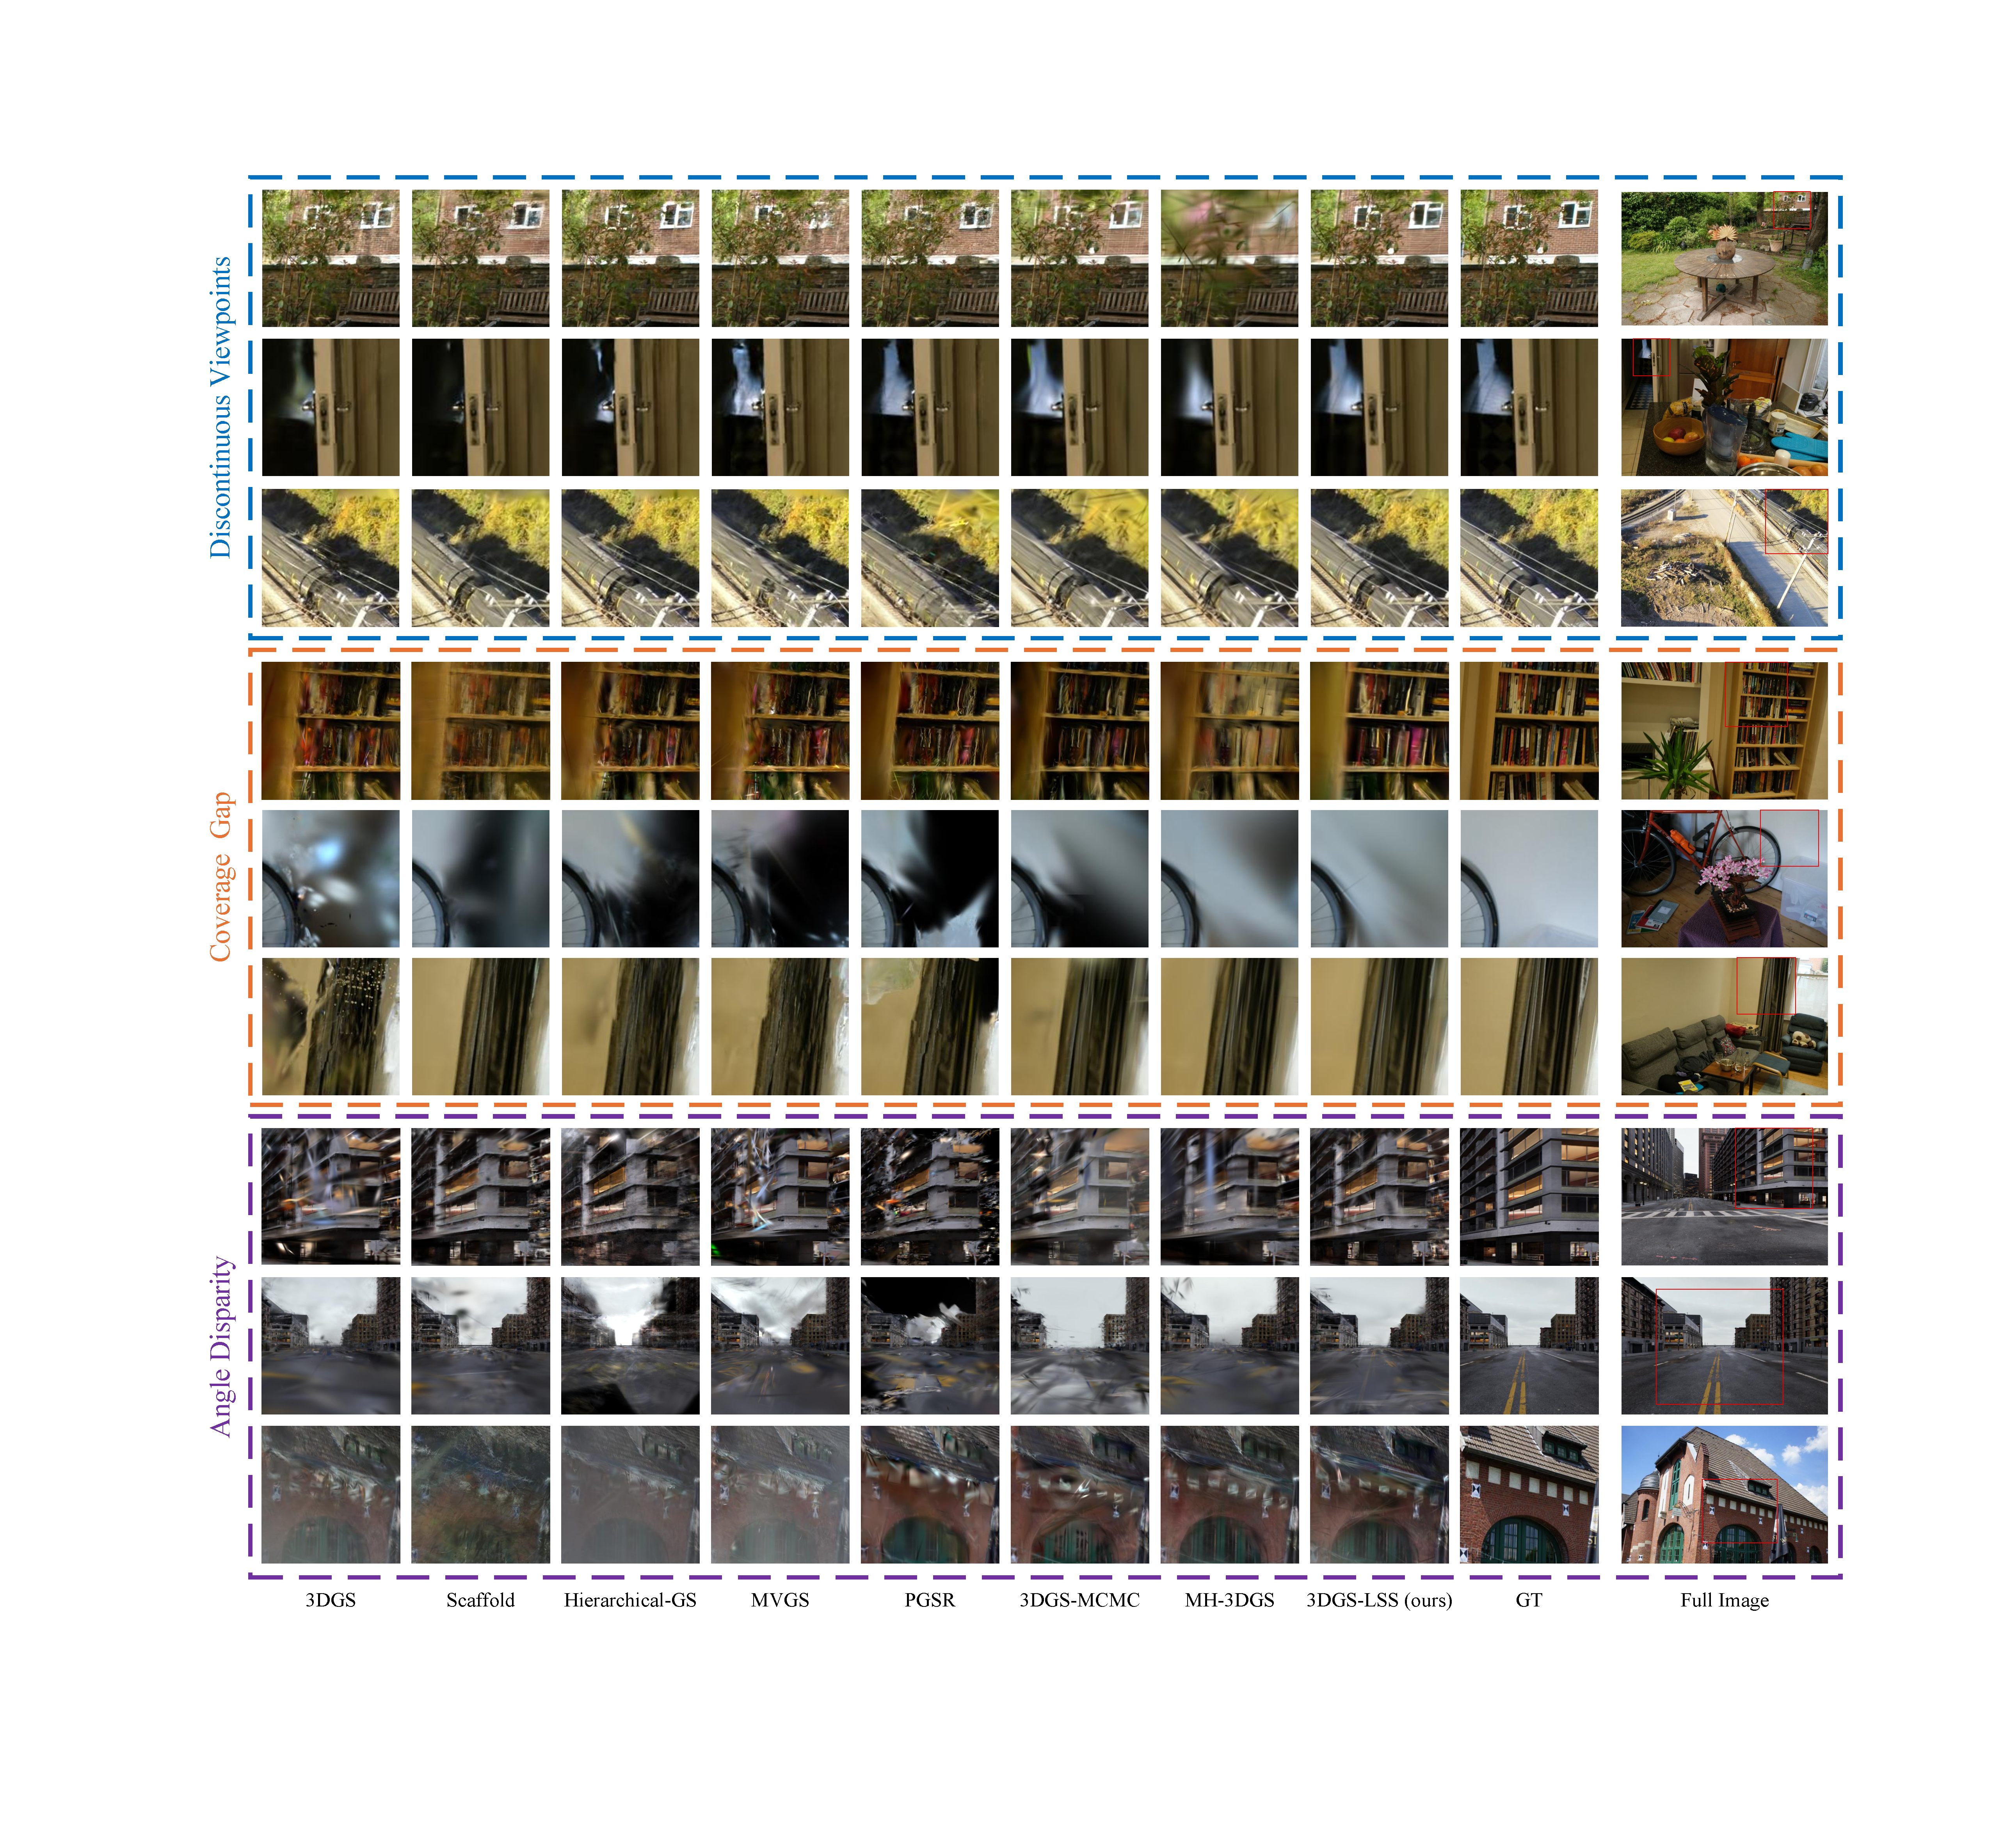
\includegraphics[width=0.96\textwidth]{pics/visual.pdf}
    \caption{Visual comparison on three biased viewpoint settings, including discontinuous trajectories, systematic coverage gaps, and viewing angle disparities.}
    \label{visual_comparison}
\end{figure*}



\subsubsection{Claim 3: CPF-guided observed-support regularization improves biased-view robustness}

Results across all three biased viewpoint settings are consistent with our third claim that CPF-guided observed-support regularization provides effective guidance for 3DGS optimization.
For example, under systematic coverage gaps (Table~\ref{tab:coverage_gap}), our method achieves the best performance across gap sizes and metrics on both Mip-NeRF 360~\cite{mipnerf360} and Tanks \& Temples~\cite{tankstemples}.
Fig.~\ref{coverage_gap_trend} further shows that our method maintains a clear advantage as the coverage gap becomes more severe. 
Under discontinuous trajectories (Table~\ref{tab:discontinuous}), 
our method obtains the best average performance across all three datasets, 
outperforming the second-best method 3DGS-MCMC~\cite{mcmc} by 0.501 dB, 0.205 dB and 0.361 dB PSNR on Mip-NeRF 360~\cite{mipnerf360}, Tanks \& Temples~\cite{tankstemples} and Mill 19~\cite{meganerf} respectively.
Under viewing angle disparities (Table~\ref{tab:angle_disparity}), our method achieves the best performance on both MatrixCity~\cite{matrixcity} and Zeche~\cite{isprs}, improving the PSNR over the second-best baseline by 0.468 dB and 0.176 dB, respectively.

The performance rankings further support the design of GS-LSS. The improvement over deterministic-only methods, such as 3DGS~\cite{3dgs} and Scaffold-GS~\cite{scaffold}, supports the view that photometric optimization alone is insufficient under biased viewpoints.
The improvement over geometric methods, such as Hierarchical-GS~\cite{hierarchical}, MVGS~\cite{mvgs} and PGSR~\cite{pgsr}, 
suggests that observation-driven regularization alone may not provide sufficient scene-level guidance under biased viewpoints. 
The improvement over MCMC-based methods, such as 3DGS-MCMC~\cite{mcmc} and MH-3DGS~\cite{mh3dgs}, indicates that
% stochasticity alone provides limited global exploration. 
stochasticity alone provides limited exploration beyond photometric gradients. 
Instead, CPF-guided observed-support regularization provides explicit guidance for 3DGS optimization, helping mitigate perspective overfitting and improve novel view synthesis under various biased viewpoint scenarios. 

Qualitative results in Fig.~\ref{visual_comparison} further support the advantages of GS-LSS. Our method produces more coherent geometry, sharper textures and fewer artifacts in unseen regions than the competitors, consistent with the reduced free-space floater density in Fig.~\ref{perspective_overfitting}. 


% \subsubsection{Summary}

% These experimental results confirm our three core claims, and lead to the following conclusions. 
% First, biased viewpoint sampling induces optimization bias in 3DGS, which leads to perspective overfitting and incomplete scene recovery. 
% Second, hand-crafted stochasticity improves the global awareness of 3DGS, but its effect is limited as the optimization lacks explicit global constraints. 
% Third, GS-LSS tackles the missing global constraints by imposing explicit global guidance through the alignment between the Gaussian primitives and the scene distribution.
% The superior performance of our method across all three biased viewpoint scenarios validates these claims and demonstrates the effectiveness of our method in improving the robustness of 3DGS under biased viewpoints.


\subsection{Ablation Study}

We conduct ablations on floater reduction, LSS parameterization, CPF construction, and stochastic optimization stability.


\subsubsection{Free-space Floater Ratio}

\begin{table}[h]
\centering
\caption{Free-space floater ratio (FFR, \%) on Mip-NeRF 360~\cite{mipnerf360} under systematic coverage gaps. Lower is better.}
\label{tab:ffr}
\scriptsize
\setlength{\tabcolsep}{4pt}
\resizebox{\columnwidth}{!}{%
\begin{tabular}{lcccccc}
\toprule
Method & 20$^\circ$ & 40$^\circ$ & 60$^\circ$ & 80$^\circ$ & 100$^\circ$ & Avg. \\
\midrule
3DGS~\cite{3dgs} & 3.914 & 3.918 & 3.932 & 3.866 & 3.792 & 3.884 \\
Scaffold-GS~\cite{scaffold} & 11.852 & 11.818 & 12.287 & 12.098 & 12.469 & 12.105 \\
Hierarchical-GS~\cite{hierarchical} & 12.129 & 12.165 & 18.589 & 12.357 & 11.725 & 13.393 \\
MVGS~\cite{mvgs} & 13.967 & 13.568 & 13.024 & 13.091 & 12.692 & 13.268 \\
PGSR~\cite{pgsr} & 14.638 & 14.732 & 15.381 & 14.618 & 15.985 & 15.071 \\
3DGS-MCMC~\cite{mcmc} & 7.596 & 7.263 & 7.557 & 7.142 & 7.091 & 7.330 \\
MH-3DGS~\cite{mh3dgs} & 3.842 & 4.104 & 3.715 & 3.753 & 3.741 & 3.831 \\
\midrule
GS-LSS (Ours) & \textbf{1.867} & \textbf{2.223} & \textbf{2.723} & \textbf{2.382} & \textbf{3.028} & \textbf{2.445} \\
\bottomrule
\end{tabular}%
}
\end{table}

We ablate free-space floater ratio (FFR) on Mip-NeRF 360~\cite{mipnerf360} under systematic coverage gaps to examine whether GS-LSS reduces support structural floaters. FFR is defined as the opacity-weighted percentage of Gaussian centers farther than 1.5\% of the scene diagonal from training-view SfM support inside the evaluated gap region. Since this CPF-independent metric is an SfM-based proxy, we use it only as a relative indicator of unsupported primitives in the weakly observed region shown in Fig.~\ref{perspective_overfitting}. Results in Table~\ref{tab:ffr} show that GS-LSS achieves the lowest average FFR across all gap sizes. This ablation supports the claim that CPF-guided optimization reduces unsupported free-space primitives, while Table~\ref{tab:ablation_LSS} further identifies which update and observed-support components contribute to this behavior.

\subsubsection{LSS Component Ablation}


\begin{table}[h]
    \centering
    % \caption{Ablation studies of LSS parameterization and random batch training,
    \caption{Ablation studies of LSS parameterization, 
    evaluated on MatrixCity~\cite{matrixcity}. Best results highlighted in bold.}
    \label{tab:ablation_LSS}
    \resizebox{\columnwidth}{!}{%
    \begin{tabular}{llccc}
        \toprule
        Method & Ablation & SSIM $\uparrow$ & PSNR $\uparrow$ & LPIPS $\downarrow$ \\
        \midrule
        \multicolumn{5}{c}{\textbf{Ablation on LSS Parameterization}} \\
        \midrule
        $\mathcal{N}(0, \sigma_{mc})$              & w/o $f_{\theta}$, w/o $g_{\theta}$ & 0.586 & 16.225 & 0.480 \\
        $\mathcal{N}(0, \sigma_{\theta})$          & w/o $f_{\theta}$, w/ $g_{\theta}$  & \textbf{0.609} & 16.544 & 0.474 \\
        $\mathcal{N}(\mu_{\theta}, \sigma_{mc})$   & w/ $f_{\theta}$, w/o $g_{\theta}$  & 0.594 & 16.599 & 0.478 \\
        $\mathcal{N}(\mu_{\theta}, \sigma_{\theta})$ & w/ $f_{\theta}$, w/ $g_{\theta}$ & 0.592 & \textbf{16.693} & \textbf{0.470} \\
        % \midrule
        % \multicolumn{5}{c}{\textbf{Ablation on Random Batch Training}} \\
        % \midrule
        % $\mathcal{N}(\mu_{\theta}, \sigma_{\theta})$ & 1 view  & 0.592 & 16.693 & 0.470 \\
        % $\mathcal{N}(\mu_{\theta}, \sigma_{\theta})$ & 2 views & 0.592 & 16.799 & 0.466 \\
        % $\mathcal{N}(\mu_{\theta}, \sigma_{\theta})$ & 3 views & \textbf{0.594} & \textbf{16.951} & \textbf{0.462} \\
        \bottomrule
    \end{tabular}%
    }
\end{table}

We ablate the two main components of the proposed LSS process, namely the CPF network $f_{\theta}$ and the variance network $g_{\theta}$, with results presented in Tab.~\ref{tab:ablation_LSS}.
In the table, 3DGS-MCMC~\cite{mcmc} is denoted by $\mathcal{N}(0, \sigma_{mc})$, where $\sigma_{mc}$ is the hand-crafted variance. For the $\mathcal{N}(0,\sigma_{\theta})$ (without CPF), the support input is replaced by a constant and the gate is conditioned on opacity and Gaussian state only. Replacing the hand-crafted variance with this learned stochastic proposal improves SSIM, PSNR, and LPIPS over the MCMC-variance row, indicating that adaptive stochasticity is beneficial under biased viewpoints. Introducing the CPF-conditioned mean term $\mu_{\theta}$ while keeping the original variance, denoted by $\mathcal{N}(\mu_{\theta}, \sigma_{mc})$, improves PSNR over both variance-only rows, indicating that the CPF model provides observed-support guidance beyond pixel-wise supervision. The full LSS process, denoted by $\mathcal{N}(\mu_{\theta}, \sigma_{\theta})$, achieves the best PSNR and LPIPS, while the learned-variance-only variant obtains the highest SSIM. This suggests that CPF drift improves photometric fidelity and artifact suppression, whereas stochastic adaptation better preserves local structural similarity.


\subsubsection{CPF Construction Sensitivity}

\begin{table}[h]
\centering
\caption{Ablation studies of geometric field and CPF model, evaluated on Tanks \& Temples~\cite{tankstemples} with coverage gap of 60$^\circ$.}
\label{tab:ablation_CPF}
\resizebox{\columnwidth}{!}{%
\begin{tabular*}{0.932\columnwidth}{@{\extracolsep{\fill}}lccc}
\toprule
{Ablation} & {SSIM} $\uparrow$ & {PSNR} $\uparrow$ & {LPIPS} $\downarrow$ \\
\midrule
\multicolumn{4}{c}{\textbf{Ablation on DBSCAN $\epsilon$ value}} \\
\midrule
$\epsilon = 0.1$  & 0.7058 & 19.1690 & \textbf{0.2458} \\
$\epsilon = 0.25$ & \textbf{0.7112} & \textbf{19.4428} & 0.2461 \\
$\epsilon = 0.5$  & 0.7058 & 19.1871 & 0.2485 \\
$\epsilon = 0.75$ & 0.7048 & 18.9888 & 0.2527 \\
$\epsilon = 1.0$  & 0.7004 & 18.9240 & 0.2550 \\
\midrule
\multicolumn{4}{c}{\textbf{Ablation on Network Architecture of CPF Model}} \\
\midrule
MLP & 0.7070 & 19.2183 & 0.2463 \\
SIREN-style & \textbf{0.7112} & \textbf{19.4228} & \textbf{0.2461} \\
\bottomrule
\end{tabular*}%
}
\end{table}


The effectiveness of the CPF model determines the quality of $\mu_{\theta}$. 
We therefore ablate two deciding factors of the CPF model, 
namely the probabilized geometric field and the CPF network architecture.
Since the density and accuracy of the geometric field are determined by the DBSCAN parameter $\epsilon$ which controls the maximum neighborhood distance, we first ablate different $\epsilon$ values to assess the effect of geometric field quality on CPF performance.
Results in Table~\ref{tab:ablation_CPF} show that performance peaks around $\epsilon = 0.25$ and gradually drops as $\epsilon$ increases, except for $\epsilon = 0.1$.
This trend has two likely causes.
First, when $\epsilon$ is below a certain threshold, DBSCAN fails to capture sufficient clusters, leading to too sparse or even empty geometric field that dampens CPF supervision.
Second, larger $\epsilon$ values commonly lead to noisier clusters, which may introduce inaccurate guidance for CPF training. 
Based on these observations, we choose $\epsilon = 0.25$ for the best overall performance trade-off.

The second part of Table~\ref{tab:ablation_CPF} compares different network architectures for the CPF model. The SIREN~\cite{implicit}-style network achieves slightly better performance than a standard MLP, which suggests that CPF training is not highly sensitive to the network design. Given this advantage at a comparable model size, we adopt the SIREN-style network in our method.


\subsubsection{LSS Stochastic Stability}

\begin{table}[h]
\centering
\caption{Results over five independent trials on Tanks \& Temples~\cite{tankstemples} with a 60$^\circ$ coverage gap.}
\label{tab:detailed_metrics}
\setlength{\tabcolsep}{4pt}
\resizebox{\columnwidth}{!}{%
\begin{tabular*}{0.932\columnwidth}{@{\extracolsep{\fill}}lccc}
\toprule
Trial & SSIM $\uparrow$ & PSNR $\uparrow$ & LPIPS $\downarrow$ \\
\midrule
Trial 1 & 0.7052 & 19.3795 & 0.2476 \\
Trial 2 & 0.7030 & 19.1766 & 0.2514 \\
Trial 3 & 0.7070 & 19.3917 & 0.2486 \\
Trial 4 & 0.7040 & 19.3068 & 0.2461 \\
Trial 5 & 0.7075 & 19.3454 & 0.2474 \\
\midrule
Mean     & 0.7053 & 19.3200 & 0.2482 \\
Variance & 3.68 $\times$ 10$^{-6}$ & 0.0075 & 3.95 $\times$ 10$^{-6}$ \\
\bottomrule
\end{tabular*}%
}
\end{table}

To evaluate the sensitivity of our method to stochastic optimization, we repeatedly train GS-LSS with the same settings for five independent trials. Results in Table~\ref{tab:detailed_metrics} show only minor performance fluctuations across trials. The PSNR of each trial stays within approximately $\pm 0.15$ dB of the mean, while the SSIM and LPIPS variances remain on the order of $10^{-6}$. These results indicate that our method exhibits stable optimization behavior despite its stochastic nature.


\subsubsection{Efficiency Trade-off}


% \begin{table}[h]
% \centering
% \caption{Average training time and rendering quality comparison on Tanks \& Temples~\cite{tankstemples} with a 60$^\circ$ coverage gap.}
% \label{tab:training-time}
% \setlength{\tabcolsep}{3pt}
% \resizebox{\columnwidth}{!}{%
% \begin{tabular*}{\columnwidth}{@{\extracolsep{\fill}}lcccc}
% \toprule
% Method & PSNR $\uparrow$ & SSIM $\uparrow$ & Time (min) $\downarrow$ & vs. 3DGS \\
% \midrule
% 3DGS        & 18.651 & 0.695 & 14.00 & 1.00$\times$ \\
% Scaffold-GS & 18.658 & 0.692 & 18.02 & 1.29$\times$ \\
% Hierarchical-GS & 18.728 & 0.694 & 14.68 & 1.05$\times$ \\
% 3DGS-MCMC   & 18.973 & 0.702 & 17.37 & 1.24$\times$ \\
% MH-3DGS     & 17.404 & 0.649 & \textbf{13.88} & \textbf{0.99}$\times$ \\
% MVGS        & 18.323 & 0.668 & 70.23 & 5.02$\times$ \\
% PGSR        & 18.020 & 0.687 & 37.35 & 2.67$\times$ \\
% \midrule
% GS-LSS (Ours)        & \textbf{19.345} & \textbf{0.709} & 38.76 & 2.77$\times$ \\
% \bottomrule
% \end{tabular*}%
% }
% \end{table}

% % Table~\ref{tab:training-time} shows that our method takes an average of 38.76 minutes for training, approximately 2.77$\times$ the training time of vanilla 3DGS~\cite{3dgs}.
% Table~\ref{tab:training-time} reports training loop wall time of different methods. It shows that our method takes an average of 38.76 minutes for training, approximately 2.77$\times$ the training time of vanilla 3DGS~\cite{3dgs}.
% This additional training time mainly arises from the CPF training, CPF queries, and the per-primitive LSS updates. 
% The cost is comparable to PGSR~\cite{pgsr} (37.35 minutes, 2.67$\times$) and lower than MVGS~\cite{mvgs} (70.23 minutes, 5.02$\times$), while achieving higher PSNR and SSIM under biased viewpoints. 
% For inference, the CPF and stochastic heads are disabled, so the training overhead does not affect rendering speed.
% We therefore consider the training cost as a reasonable trade-off for the challenging biased viewpoint scenarios, where reconstruction fidelity and synthesized view quality matter more than training speed.

\begin{table}[h]
\centering
\caption{Relative training cost and rendering quality comparison on Tanks \& Temples~\cite{tankstemples} with a 60$^\circ$ coverage gap. Training cost is normalized by vanilla 3DGS.}
\label{tab:training-time}
\setlength{\tabcolsep}{3pt}
\resizebox{\columnwidth}{!}{%
\begin{tabular*}{\columnwidth}{@{\extracolsep{\fill}}lcccc}
\toprule
Method & PSNR $\uparrow$ & SSIM $\uparrow$ & LPIPS $\downarrow$ & Time vs. 3DGS $\downarrow$ \\
\midrule
3DGS        & 18.651 & 0.695 & 0.269 & 1.00$\times$ \\
Scaffold-GS & 18.658 & 0.692 & 0.269 & 1.29$\times$ \\
Hierarchical-GS & 18.728 & 0.694 & 0.267 & 1.05$\times$ \\
3DGS-MCMC   & 18.973 & 0.702 & 0.257 & 1.24$\times$ \\
MH-3DGS     & 17.404 & 0.649 & 0.291 & 0.99$\times$ \\
PGSR        & 18.020 & 0.687 & 0.295 & 2.67$\times$ \\
MVGS        & 18.323 & 0.668 & 0.275 & 5.02$\times$ \\
\midrule
GS-LSS (Ours)        & \textbf{19.345} & \textbf{0.709} & \textbf{0.247} & 2.77$\times$ \\
\bottomrule
\end{tabular*}%
}
\end{table}


Table~\ref{tab:training-time} reports the quality-cost trade-off with training cost normalized by vanilla 3DGS~\cite{3dgs}. 
Under the same 60$^\circ$ coverage-gap protocol, GS-LSS achieves the best PSNR, SSIM, and LPIPS at 2.77$\times$ the 3DGS training time. 
This cost is comparable to PGSR~\cite{pgsr} (2.67$\times$) and substantially below MVGS~\cite{mvgs} (5.02$\times$), while GS-LSS yields higher rendering quality than both. 
The extra time mainly comes from CPF training, CPF queries, and per-primitive LSS updates, which target weakly observed regions where biased training causes the largest degradation. 
These modules are used only during training. At inference, the CPF and stochastic heads are disabled, and rendering uses the standard optimized Gaussian field. 
We therefore view GS-LSS as a reasonable one-time training investment when held-out view fidelity and artifact suppression matter more than raw training speed.


\section{Limitations}

GS-LSS regularizes Gaussian primitives toward aggregated observed support, but it does not recover geometry that is completely unsupported by the input views. The CPF field is derived from filtered in-training geometry, so its reliability depends on the quality of the stabilized Gaussian field and the effectiveness of outlier filtering. The method also increases training cost because of the CPF supervision and queries. Reducing this cost and improving CPF reliability under extremely sparse captures are important directions for future work.


\section{Conclusion}

% We present GS-LSS, an observed-support regularized learned stochastic optimization framework for Gaussian Splatting under biased viewpoints. Rather than relying solely on view-dependent photometric supervision, GS-LSS aligns Gaussian primitives with an aggregated observed-support field through a Learned Stochastic Sampling process. Its Continuous Probability Field estimates observed support from globally aggregated geometric priors and provides gradient-based drift with adaptive stochastic exploration. Experiments on three biased viewpoint scenarios show strong quantitative and qualitative results among the evaluated baselines, mitigating perspective overfitting and improving observed-support consistency at moderate training overhead. Future work will improve the efficiency and reliability of support estimation while maintaining high-quality rendering. 

We present GS-LSS, an observed-support regularized learned stochastic optimization framework for Gaussian Splatting under biased viewpoints. Rather than relying solely on view-dependent photometric supervision, GS-LSS aligns Gaussian primitives with an aggregated observed-support field through a Learned Stochastic Sampling process. Its Continuous Probability Field estimates observed support from globally aggregated geometric priors and provides gradient-based drift with adaptive stochastic exploration. This scene-level guidance helps reduce perspective overfitting and encourages more globally consistent reconstruction. Experiments on three biased viewpoint scenarios show strong quantitative and qualitative results among the evaluated baselines, improving observed-support consistency at moderate training overhead. Future work will improve the efficiency and reliability of support estimation while maintaining high-quality rendering.

\section*{Acknowledgement}
This work was supported by the Guangdong Provincial Science and Technology Program under Grant No. 2023A1111120006 (Acceptance No. c23201809261900030; Document No. Yue Ke Zi Zi (2024) No. 24).

\bibliographystyle{IEEEtran}
\bibliography{citations}  % This tells BibTeX which .bib file to use


\vfill

\end{document}
